\documentclass[10pt,a4paper]{article}
\usepackage[utf8]{inputenc}
\usepackage[paper=a4paper, margin=1.5cm]{geometry}

% FA icons
\usepackage{hyperref}
\usepackage{url}
\usepackage{color}
\usepackage{xcolor}
\usepackage{graphicx}
\usepackage{tikz}
\usepackage{minted}

\setminted{
    breaklines=true,
    fontsize=\footnotesize,
    framesep=2mm
}

\usepackage{caption}
\usepackage{subcaption}

\floatplacement{figure}{H}

\DeclareCaptionLabelFormat{numeric}{příloha #2.}
\captionsetup{labelformat=numeric,labelsep=quad}

\usepackage{amsmath}
\usepackage{amssymb}

% data highlighting
\newcommand{\harddata}[1]{\boxed{\texttt{#1}}}

\hypersetup{
    colorlinks=true,
    linkcolor=blue,
    filecolor=magenta,      
    urlcolor=cyan,
    pdftitle={Bakalářská práce~--~Využití IT ke generování zadání písemných testů},
    pdfpagemode=FullScreen,
    colorlinks=false,% hyperlinks will be black
    pdfborderstyle={/S/U/W .5}% border style will be underline of width 1pt
}

% citace a jazyk
\usepackage[main=czech, english]{babel}
\usepackage{csquotes}
\usepackage{biblatex}
\addbibresource{zdroje.bib}

\begin{document}
	\begin{titlepage}
		\begin{center}
            {
            \centering
            
\includegraphics[]{./img/UP_logo_PdF-UP_horizont_cz.pdf}
            }
			
			\vspace{3cm}

            {
                \LARGE
                \textbf{Šimon Janča}\\
                3.\,ročník\\[8mm]
                Obor: Informační technologie a matematika pro vzdělávání
            }

            \vspace{4cm}
			
			{
			    \textbf{\Huge Využití IT ke generování zadání písemných testů}\\[4mm]
			    \Large
			    Bakalářská práce
			}

            \vfill
            
            {
                Vedoucí práce:
                doc. RNDr. Petr Šaloun, Ph.D.
                \hfill
    			Olomouc \the\year{}
            }
			
		\end{center}
	\end{titlepage}
	% generate table of contents
	\tableofcontents

	\newpage
    \clearpage
    \setcounter{page}{1}
	
	\section{Úvod}
    V~úvodu této práce bych~chtěl na~několika stránkách popsat nástroje, které je~možné použít pro~tvorbu testů a~definovat potřeby, které v~této souvislosti mohou nastat.
    druhé
    Ve~druhé části popíšu návrh a~implementaci moderních aplikací a~vytvořím aplikaci, kterou učitelé mohou používat k~tvorbě různých variant zadání školních testů. V~rámci toho popíšu základní prvky při~vývoji \emph{moderní \emph{MVC}} aplikace a~popíšu důvody k~jednotlivým rozhodnutím od~návrhu a~výběru technologií, přes plánování pomocí diagramů, až~k~její implementaci a~spuštění za~použití vybraných technologií.
    
    Aplikace mohou samozřejmě vznikat i~jinými způsoby, nicméně by~mělo jít o~čitelný a~reprodukovatelný postup vývoje, zabezpečení a~údržby podobné aplikace. Vyhotovená aplikace bude následně veřejně dostupná jako webová služba.

    \section{Testy, testové úlohy}

    Školní testy jsou nástrojem pro hodnocení znalostí a dovedností studentů. Vznikají tak, že~učitelé nebo vzdělávací instituce vytvářejí \emph{otázky} (\emph{problémy}~\cite{zhouf:tvorbamatproblemu}) a~úkoly, které jsou zaměřeny na~konkrétní téma nebo oblast učiva. Tyto \emph{otázky} a~úkoly jsou poté zařazeny do testu, který je studentům předložen k~vyplnění.

    Umožňují učitelům zjistit, jak dobře studenti porozuměli učivu a jaké jsou jejich silné a~slabé stránky. Testy také pomáhají studentům zjistit, na~čem by~měli pracovat, aby se~zlepšili. Kromě toho jsou výsledky různých testů použity jako parametr přijímání na~vysoké školy nebo k~udělování stipendií.
    
    Testy mohou být psány ručně, nebo mohou být generovány pomocí počítačových nástrojů. V~této kapitole se~budu zabývat problematikou testových úloh, jejich tvorbou a~možnostmi, které nám dnešní technologie nabízí.

    V~rámci této práce se~budu zabývat především písemnými testy, které jsou~používány na~základních a~středních školách, nicméně většina z~popisovaných pojmů je~použitelná i~pro~jiné typy testů.

        \subsection{Uzavřené úlohy}
        
        \emph{Uzavřené úlohy} jsou~úlohy, které mají předem danou množinu odpovědí. Respondent si~při~vyplňování testu vybere jednu z~nich (nebo více správných odpovědí~--~podle zadání) a~tím odpoví na~otázku. Může jít o~označení vyjmenovaných možností nebo z~obecně předpokládaných odpovědí, např.~na~otázku \uv{V~jakém městě bydlíte?} očekáváme v~odpovědi existující město, nikoliv několik popisných vět.

        Řešení takových úloh může~být~méně náročné, jak na~žáka, který může jednodušeji určit (nebo uhodnout) správnou odpověď, tak na~učitele, který nemusí při~hodnocení brát v~potaz různé možnosti odpovědí.

        Nabízí se~tím možnost zápisu do~odpovědních archů a~tím jednodušší vyhodnocení pomocí počítače.

        Bodování úloh může být jednoduché, kde~za~každou správnou odpověď přičteme jeden bod, nebo může být složitější, kde např.~za~každou správnou odpověď přičteme jeden bod, ale za~každou špatnou odpověď bod (nebo část bodu) odečteme, za~nevyplněnou odpověď většinou nepřičítáme ani~neodečítáme žádný bod.

        Může jít také třeba o~doplnění písmen výběrem za~účelem procvičení správné gramatiky. Také jsou možné různé doplňovačky nebo výběr správného slova do textu, např.~v~cizích jazycích. V~matematice může jít~o~výběr správné hodnoty (nebo množinu hodnot).

        \subsection{Otevřené úlohy}
        \emph{Otevřené úlohy} naopak předem dané možnosti odpovědí nemají. Respondent musí odpověď napsat sám, odpovědí může být slovo, věta, nebo třeba i~celý text. Může jít o~návodné \emph{otázky}, kde~je~potřeba odpovědět vlastními slovy, nebo o~\emph{otázky}, kde~je~potřeba vypočítat nějakou hodnotu. Můžeme tak~zhodnotit odpověď nejen podle výsledných hodnot, ale i~podle postupů, které byly~použity.

        Řešení takových úloh je~náročnější, jak na~žáka, který musí odpověď vymyslet, tak na~učitele, který musí při~hodnocení brát v~potaz různé možnosti odpovědí. Na~druhou stranu to~umožní ocenit i~částečně správné odpovědi nebo vlastní invenci při~řešení, což by~u~uzavřených úloh nebylo možné. \cite{rozhlasOUtazky}

        \subsection{Tvorba testů}
        Při tvorbě testu ze~začátku uvažujeme o~jeho rozsahu. Jde~o~obecný test, ověřující schopnosti žáka, nebo pouze konkrétního výřezu učiva daného předmětu?

        \uv{\emph{Otázky} by měly být pestré, pokrývající co nejširší spektrum prověřovaného učiva, a~to z~různých úhlů pohledu. Takže by~určitě neměly chybět \emph{otázky} zjišťující schopnost žáka pracovat s~fakty (značky a~jednotky fyzikálních veličin, matematické vyjádření fyzikálních zákonů)}. \cite{Suchoradsky:testy}
        
        Problémem je~také~tvorba správných a~nesprávných odpovědí při~tvorbě (\emph{uzavřených}) otázek. Pokud naším cílem je~dobře ověřit znalosti, pak~je~nutné tvořit \emph{otázky} tak, aby nesprávné odpovědi vypadaly věrohodně. Taky nesmíme zapomenout, aby odpovědi obsahovaly správné řešení (může být specifikováni zadáním).

        Můj~druhý obor je~matematika, proto se~v~příkladu zaměřím na~ni. Pokud budeme testovat např.~znalosti \emph{lineárních rovnic}, pravděpodobně necháme otázku s~otevřenou odpovědí, abychom zjistili, zda je~student schopný odpověď vypočítat a~jak~při~tom postupuje. Ale může nastat situace, že~chceme ověřit rychlý úsudek studenta na~základě daného učiva a~pak mu nabídneme možnosti. V~tomto případě je~potřeba, aby nesprávné možnosti vypadaly věrohodně, aby student nemohl jednoduše uhodnout správnou odpověď, ale k~odhadu využil své~znalosti.

        Možnostmi pro~odpovědi k~řešení lineární rovnice budou výsledné hodnoty proměnné (např.~$x$). Různé možnosti můžeme definovat třeba výpočtem z~koeficientů. Nebo řekněme, že~budeme chtít, aby výsledek odpovídal některému z~číselných oborů. Pro žáky, kteří neumí počítat se~zlomky budeme chtít rovnici s~celočíselným výsledkem. Naopak pokud chceme ověřit znalost výpočtu kvadratické rovnice s~komplexními čísly, budeme chtít v~rovnici a~odpovědích obsáhnout imaginární složku. \cite{zhouf:tvorbamatproblemu}

        \subsection{V současnosti používané nástroje}
        V~současnosti je~pro~účely tvorby testů používáno několik nástrojů, které se~liší svými možnostmi a~způsobem použití.
        
        Existují některé \emph{webové stránky}, které nabízejí hotové testy ke~stažení. 
        % TODO: příklady webů
        Ty~potom učitel jen~vytiskne. Na~internetu je~možné najít i~jednotlivé příklady, ze~kterých učitel test sestaví. Pokud je~potřeba procvičovat test k~přijímacím zkouškám, ochotně nám materiál poskytne \emph{CERMAT} nebo \emph{SCIO}.

        Některé učebnice, které jsou používány ve~školách, mají v~rámci verze pro~učitele didaktické přílohy ve~kterých jsou testy k~použití připravené. Taky je~možné použít některé cvičení z~pracovních listů.

        Pokud si~učitel chce test vytvořit, může používat klasické \emph{tabulkové procesory}, jako je~např.~\emph{Microsoft Excel} nebo \emph{Google Sheets}, nebo \emph{textové procesory}, jako je~např.~\emph{Microsoft Word}, \emph{LibreOffice Writer} nebo \emph{Google Docs}. Grafické zadání je~potom možné vložit do~těchto souborů.

        V~současnosti se~přímo nabízí do~tvorby otázek nebo i~celých testů zapojit \textbf{umělou inteligenci} (\emph{AI}). Pokud tedy \emph{ChatGPT}, \emph{Google Bard} nebo jinému jazykovému modelu zadáme vytvoření testových otázek na~konkrétní téma, jistě nám je~ochotně připraví.
        % TODO: zdroj?

        % TODO: doplnit podle výsledků dotazníku
        
        Také je~zde možnost otázky zapsat ručně a~zkopírovat je~pomocí tiskárny se~skenerem.

        \subsection{Co na tvorbu testů používají učitelé}
        % TODO: dotazník/rozhovory s učiteli

    \section{Vývoj moderních webových aplikací}
    V dnešní době je~webová aplikace první volbou pro~většinu vývojářů. Je~to~způsobeno tím, že~webová aplikace je~dostupná z~jakéhokoliv zařízení, které má~přístup k~internetu a~je~schopné zobrazit webový prohlížeč. Webová aplikace je~také snadno aktualizovatelná a~není potřeba ji instalovat na~každém zařízení zvlášť, stačí pouze otevřít prohlížeč na~dané adrese.
    
    Vývojáři se~také nemusí starat o~kompatibilitu s~různými operačními systémy, protože webový prohlížeč
    je~dostupný na~většině z~nich. Webová aplikace je~také snadno škálovatelná, protože je~uložena na~serveru a~uživatelé se~k~ní připojují.
    
    Navíc je možné díky různým nástrojům vydat aplikaci pro~různé platformy (Android, IOS\dots) z~jednoho zdrojového kódu.\cite{adobe:webapp}

    Většina dnešních projektů je~tedy vyvíjena jako~MVC webová \emph{aplikace}. Tím oddělíme logiku aplikace od~jejího zobrazení, což nám umožňuje vývoj funkční části aplikace nezávisle na~uživatelské části a~můžeme třeba pracovat s~různými technologiemi.
    
    Pro obě části existují připravené technologie, které nám usnadní vývoj a~umožní nám vytvořit aplikaci rychleji a~s~menším množstvím chyb.

    \uv{Pro frontend i backend aplikace existuje na webu obrovské množství použitelných materiálů. Ať už jsou to různé grafické prvky nebo serverové komponenty, to vše je už někde nejspíše hotové.}\cite{itnetworkBestPractices}

        \subsection{Základní statická HTML stránka}
        V roce 1989 vytvořil Tim Berners-Lee první webový prohlížeč a~jazyk \emph{HTML}. \emph{HTML} je~zkratka pro~HyperText Markup Language (Hypertextový značkovací jazyk). Základem je HTML stránka~--~soubor, který obsahuje textový obsah a~HTML značky, které určují význam jednotlivých částí obsahu. Navíc lze jednotlivé soubory propojit pomocí hypertextových odkazů, které umožňují uživateli kliknutím přecházet z~jedné stránky na~druhou.

        Jednotlivé \emph{HTML} stránky se~skládají z~\emph{HTML} značek (\emph{prvků}), ale i~\emph{CSS} stylů, které určují jak má prohlížeč jednotlivé prvky stránky vykreslit uživateli. K~tomu se~přidává i~JavaScript, který umožňuje přidat do~stránky dynamický obsah a~reagovat na~uživatelské akce jako kliknutí myši nebo~odeslání formuláře. \cite{berners:1989:proposal}

        Jednotlivé prvky je možné také označit pomocí \emph{identifikátorů} a~\emph{tříd}, které se~používají pro~jejich identifikaci ve~stránce. Zatímco \emph{tříd} může mít prvek více, identifikátor může být~použit v~dokumentu pouze jednou~--~měl by~být unikátní. \emph{Třídy} se~používají pro~označení skupiny prvků, které mají mít stejný vzhled nebo funkcionalitu. Prvek může mít více \emph{tříd} a~kombinovat tak jejich vlastnosti. \cite{jpw:tridy}

        \subsection{HTML s dynamickým obsahem}
        HTML stránky mohou mít i~dynamický obsah. To znamená, že~se~mohou měnit podle toho, jak s~nimi uživatel pracuje. Na~úrovni serveru se~může generovat \emph{HTML} stránka, která obsahuje dynamický obsah. V~dnešní době je~oblíbený přístup generovat výslednou stránku pomocí \emph{javascriptu} až~na~straně uživatele a~od~\emph{serveru} si~vyžádat pouze data, nicméně v minulosti se~dynamický obsah generoval převážně na~serveru pomocí technologií jako~\emph{PHP (HyperText Preprocessor)}, \emph{ASP.NET}, které na~serveru vygenerovaly kompletní \emph{HTML kód} stránky i~s~načtenými daty.

        To samozřejmě znamenalo, že~při~každé změně obsahu bylo~potřeba znovu kontaktovat server a~stránku znovu načíst do~prohlížeče. Také byla veškerá komunikace omezená na~požadavek od~klienta, server pouze obsluhoval požadavky a~neměl možnost samostatně zaslat zprávu klientovi. Tento problém právě adresuje Javascript. Odesílá požadavky na~server a~na~základě odpovědi mění obsah celé nebo části stránky. Díky metodám, jako je~\emph{AJAX (Asynchronous Javascript And XML)}~\cite{ajax:mdn} je~možné komunikovat se~serverem i~bez~načítání celé stránky.

        To~znamená, že~když např.~uživatel klikne na~tlačítko, nemusí se~stránka znovu načítat celá, pouze se~načtou data ze~serveru a~na~stránce se~upraví~obsah. To~je~rychlejší a~příjemnější pro~uživatele.

        Server může~--~samozřejmě po~povolení ze~strany uživatele~--~zasílat zprávy na~klientské zařízení a~vyžádat si~nějakou akci, díky \emph{Server-Sent Events}~\cite{sse:mdn} nebo udržovat spojení pomocí \emph{WebSockets}. Příkladem použití \emph{WebSockets} mohou být živý přenos videa, online hry, internetové hovory nebo jiné prvky na~webu, kde~využijeme oboustranou komunikaci.~\cite{websocket:mdn}

        \subsection{Kompilátor a interpret}
        Pro~lepší pochopení programování aplikací je~potřeba si~ujasnit rozdíl mezi kompilovaným a~interpretovaným jazykem.

        \textbf{Kompilovaný} jazyk je~jazyk, který se~pomocí tzv.~překladače (\emph{kompilátoru}) překládá do~binárního souboru, který obsahuje přímo instrukce pro~procesor. Při~každém spuštění se~potom do~paměti načte binární soubor s~instrukcemi a~procesor je~vykonává.
        
        Při~překladu (\emph{kompilaci}) překladač navíc kontroluje správnost zápisu a~případné zjistitelné chyby vypíše. To~umožňuje odhalit chyby před spuštěním programu.

        \emph{Kompilátor} navíc při~překladu provádí optimalizace, které zvyšují výkon a~snižují nároky programu na~\emph{hardware}.

        \textbf{Interpretovaný} jazyk je~naopak vykonáván programem, kterému říkáme interpret. Ten~čte~příkazy a~přímo je~vykonává. To~znamená, že~při~každém spuštění se~příkazy překládají znovu. Navíc je~interpret program, který musí běžet, zatímco příkazy interpretuje, což je taky jeden z~důvodů, proč bývají interpretované jazyky pomalejší a~náročnější na~využítí zdrojů, než~kompilovaný.
        
        Interpretování může ale přinést i~výhody. Například je~možné příkazy vykonávat ihned, bez~nutnosti překladu a~není potřeba obstarávat správu paměti. \cite{ueda:compiled}
        
        \subsection{Překladač (kompilátor)}
        Překladač je~program, který čte~zdrojový kód a~překládá ho do~podoby binárního souboru, který obsahuje instrukce vykonávané procesorem. Překladač také kontroluje správnost zápisu a~případné zjistitelné chyby vypíše. To~umožňuje odhalit některé chyby ještě před~spuštěním výsledného programu.
        \emph{Překladače} i~\emph{interprety} pracují v~několika fázích:
        \begin{enumerate}
            \item \textbf{Lexikální analýza}~--~\emph{kompilátor} čte zdrojový kód znak po~znaku a~rozděluje~jej na~jednotlivé \emph{tokeny} a~určuje jejich typ (slova, čísla, operátory\dots). Při~tom kontroluje správnost zápisu a~případné chyby vypíše. Výstupem je~seznam tokenů.
            \item \textbf{Syntaktická analýza}~--~kontroluje, jestli jsou jednotlivé \emph{tokeny} správně strukturovány a~v~jakém vztahu k~sobě stojí. Generuje \emph{abstraktní syntaktický strom (AST = Abstract Syntax Tree)}, který reprezentuje strukturu programu.
            \item \textbf{Sémantická analýza}~--~kontroluje správnost použití jednotlivých \emph{tokenů} a~jejich význam. Generuje tabulku symbolů, která obsahuje informace o~proměnných a~funkcích, dostupných v~programu.
            \item \textbf{Optimalizace}~--~v~této fázi optimalizujeme kód, aby byl ve~výsledku rychlejší a~méně náročný na~procesor. Optimalizace se~děje v~závislosti na~použitém jazyce a~překladači a~může být~prováděna několikrát v~různých fázích překladu (a~nemusí být prováděna vůbec).
            \item \textbf{Generování kódu}~--~Když~máme \emph{AST}, můžeme generovat výslednou podobu programu nebo dat v~požadované formě~--~binární soubor programu, optimalizovaný bytecode pro spouštění pomocí interpretu, program zapsaný v~jiném jazyce nebo interpretujeme jako~jinou formu dat.
        \end{enumerate} \cite{baeldungCompilersWork}

        \subsection{Procedurální a~objektově orientované programování (OOP)}
        \emph{Procedurální programování} je~způsob programování, kdy se~program skládá z~jednotlivých procedur, které se~volají za~sebou. Procedura je~část programu, která vykonává určitou činnost. Procedury mohou mít parametry, které jim předáváme při~volání. Procedury mohou volat jiné procedury, což umožňuje znovupoužití kódu. Procedury a~funkce jsou~si~podobné, kromě faktu, že~funkce vždy vrací (\texttt{return}) nějakou hodnotu, zatímco procedura pouze vykoná své~instrukce.
        % TODO: najít zdroj (mimo wiki)
        
        V~dnešní době se~častěji používá \emph{OOP}, protože umožňuje vývojáři programovat v~abstraktnější rovině a~tím zjednodušit vývoj a~údržbu programu. Jednotlivé objekty představují \uv{modely} objektů z~reálného světa, což~je~pro~člověka přirozenější způsob myšlení. Při~práci v~týmu je~také jednodušší rozdělit si~práci na~jednotlivé části programu, na~kterých mohou vývojáři pracovat paralelně.
        
        \emph{OOP (objektově orientované programování)} je~programovací paradigma, které se~snaží modelovat objekty z~reálného světa. V~OOP se~program skládá z~objektů, které mají své~vlastnosti a~metody (funkce). \emph{Objekty} vytváříme ze~tříd, což~jsou jakési vzory, podle kterých se vytvářejí (\emph{inicializují})~objekty. \emph{OOP} má 4~základní vlastnosti, které při vývoji využíváme; \cite{Keogh:OOP}
        \begin{itemize}
            \item \textbf{Zapouzdření}~--~objekty mohou své~vlastnosti a~metody, skrýt před~okolním světem. To~umožňuje měnit vnitřní strukturu objektu bez~nutnosti měnit ostatní části programu.
            \item \textbf{Dědičnost}~--~objekty mohou dědit vlastnosti a~metody od~jiných objektů. To~umožňuje znovupoužití kódu a~zjednodušení programu.
            \item \textbf{Polymorfismus}~--~objekty mohou mít stejné~vlastnosti a~metody, ale mohou se~lišit v~implementaci. To~umožňuje vytvářet obecné~třídy, které mohou být použity pro~více konkrétních případů.
            \item \textbf{Abstrakce}~--~třídy mohou být \emph{abstraktní}, což~znamená, že~nemusí být~implementována jejich funkcionalita a~nelze je~samostatně \emph{inicializovat}. To~umožňuje vytvářet obecné (tzv.\emph{bázové})~třídy, které mohou být použity jako vzor pro~odvození jiných konkrétních tříd, využívajících jejich vlastnosti a~metody.
        \end{itemize}
        % TODO: prověřit abstrakci

        Jazyk~\emph{Go} (Golang) podporuje~\emph{OOP} pouze~částečně. Je~nutné si~uvědomit, že~jde o~jazyk \emph{strukturovaný}, nikoliv \emph{objektově orientovaný}. Některých vlastností \emph{OOP} ale můžeme dosáhnout pomocí použití \emph{struktur} a~\emph{rozhrání} (\emph{interface}). Metody na~strukturách můžeme vytvořit za~pomocí \emph{funkcí na~struktuře} (\emph{receiver function})
        Výraz \emph{rozhrání} běžně definuje komunikaci mezi objekty, viz.~kapitola věnovaná~\emph{API}. V~případě \emph{OOP} definují vzor, podle kterého je~potřeba implementovat budoucí třídy. \cite{go:OOP}
        
        A \emph{Javascript} je sice považován za \emph{objektově orientovaný}, nicméně \emph{OOP} implementuje formou tzv.~prototypové dědičnosti, nikoliv tradičním použitím tříd. V praxi tak má každý objekt definovanou vlastnost \texttt{proto}, která buďto obsahuje rodičovský objekt nebo obecný prototyp objektů. \cite[2.1.01]{kantor_javascript}
        
        V~příkladě \ref{oop:difference} je~pro~porovnání ta~samá funkcionalita zapsána v~jazyce \emph{Javascript} pomocí \emph{tříd} a~v~jazyce \emph{Go} pomocí \emph{struktur}, \emph{rozhraní} a~tzv.~\emph{receiver function}, což~jsou funkce definované na~dané struktuře (podobně jako \emph{metody} ve~třídě). \emph{Interface} (rozhraní) zajišťují kontrolu, že~na~daném typu~existují požadované \emph{metody}. Je~tak~možné kontrolovat, že~objekt, který vyšetřujeme má~požadované vlastnosti a~metody, a~můžeme jej~používat zamýšleným způsobem např.~ve~funkci.~\cite{go:OOP}

        \begin{figure}
            \begin{subfigure}[b]{0.45\linewidth}
                \begin{minted}{js}
class Animal {
    constructor(name) {
        this.name = name;
    }

    makeSound() {
        if (!this.sound) {
            const name = this.constructor.name;
            console.log(`What does the ${name} say?`);
            return;
        }
        console.log(`My name is ${this.name} and I go ${this.sound}`);
    }
}

class Dog extends Animal {
    constructor(name) {
        super(name);
        this.sound = "Haf";
    }
}

class Cat extends Animal {
    constructor(name) {
        super(name);
        this.sound = "Mňau";
    }
}

class Fox extends Animal {}

const a = new Dog("Alík");
a.makeSound();
const b = new Cat("Micka");
b.makeSound();
const c = new Fox("Foxy");
c.makeSound();
                \end{minted}
                \caption{Zápis pomocí tříd v Javascriptu}
            \end{subfigure}
            \hfill
            \begin{subfigure}[b]{0.45\linewidth}
                \begin{minted}{go}
import "fmt"

// Animal is an abstract class (interface) in Go
type Animal interface {
	makeSound()
}

// AnimalBase is a base struct to store common properties of animals
type AnimalBase struct {
	sound string
	name  string
}

// Type (struct) representing a dog
type Dog struct {
	AnimalBase
}

// Cat
type Cat struct {
	AnimalBase
}

// Constructor-like function to create an instance of AnimalBase
func NewAnimalBase(name string) *AnimalBase {
	return &AnimalBase{
		name: name,
	}
}

// Method implemented for AnimalBase, which all animals inherit
func (a *AnimalBase) makeSound() {
	fmt.Printf("My name is %s and I go %s\n", a.name, a.sound)
}

// NewDog je tzv. konstruktor objektu Dog, vytvoří v paměti strukturu s konkrétními daty o psovi (jméno) a vrátí ukazatel na dané místo v paměti
func NewDog(name string) *Dog {
	dog := &Dog{
		AnimalBase: *NewAnimalBase(name),
	}
	dog.sound = "Haf"
	return dog
}

// NewCat je konstruktor objektu Cat, vytvoří strukturu s konkrétními daty o kočce
func NewCat(name string) *Cat {
	cat := &Cat{
		AnimalBase: *NewAnimalBase(name),
	}
	cat.sound = "Mňau"
	return cat
}

// a musí implementovat rozhrání (interface) Animal
func animalMakeSound(a Animal) {
    a.makeSound()
}

func main() {
	a := NewDog("Alík")
	animalMakeSound(a)

	b := NewCat("Micka")
	animalMakeSound(b)
}
                \end{minted}
                \caption{Stejná funkcionalita v jazyce Go}
            \end{subfigure}
            \caption{Zápis OOP v PHP je stručnější než v Go}
            \label{oop:difference}
        \end{figure}

        \subsection{Javascript}
        \emph{Javascript} je~\emph{skriptovací} jazyk, který se~používá k~tvorbě interaktivních webových stránek. Dokáže reagovat na~uživatelské akce, jako je~kliknutí, a~tedy na~rozdíl od~statické podoby \emph{HTML} stránky dokáže měnit obsah podle toho, jak~uživatel se~stránkou pracuje bez~nutnosti nového požadavku na~server.

        Vznikl v~roce 1995 a~jeho tvůrci jsou \emph{Brendan Eich} a~společnost \emph{Netscape}. \emph{Javascript} (resp.~\emph{Typescript}) je~podle~--~průzkumů síte \textbf{Stack Overflow}~--~v~současnosti nejpoužívanějším programovacím jazykem na~světě používaným nejen pro~tvorbu webových aplikací, ale i~pro~tvorbu \emph{nativních} a~dokonce některých \emph{embedded} aplikací, což jsou programy určené pro~konkrétní elektronická zařízení s~konkrétním účelem, např.~rozhrání pro~dotyková zařízení (GPS, televize, kontrolní panel v~autě ap.).

        Díky spouštěčům Javascriptu, kterým říkáme \emph{Javascriptové enginy}, je~možné spouštět Javascript na~různých platformách. A~tak~můžeme Javascript spouštět v~prohlížeči, ale i~na~serveru nebo dokonce na~mikrokontrolerech. Jeden jazyk tak~zvládne pokrýt většinu potřeb, které může autor aplikace při~vývoji mít.

        \emph{Javascript} dokáže příkazy zpracovávat \emph{synchronně} (sekvenčně) i~\emph{asynchronně} (paralelně). \textbf{Synchronní} zpracování znamená, že~se~příkazy vykonávají postupně, tak, jak jsou zapsány ve~skriptu. \textbf{Asynchronní} zpracování naopak znamená, že~se~příkazy vykonávají nezávisle na~sobě, tedy ke~spuštění dalšího příkazu nečekáme na~dokončení předchozího. To~je~užitečné např.~při~načítání dat ze~serveru, které může trvat delší dobu. V~tomto případě je~možné spustit \emph{asynchronní akce} a~pokračovat ve~zpracování sekvence příkazů programu. Když dojde k~dokončení \emph{asynchronní akce}, vykoná~se příkaz, který na~její dokončení čeká. V~rámci \emph{asynchronní operace} můžeme čekat na~dokončení více akcí. \cite{kantor_javascript}

        Zpracování \emph{Javascriptu} je~rozděleno do~dvou částí. První částí je~\emph{Javascriptový engine}, který zpracovává Javascriptový kód a~podle toho spouští instrukce. Druhou částí jsou~tzv.~\emph{Web APIs}, které umožňují využívat funkce prohlížeče a~systému. Jde~o~instrukce, poskytované nikoliv Javascriptovým enginem, ale prohlížečem nebo systémem. Jde~např.~o~přístupu k~\emph{DOMu}, kameře, mikrofonu nebo veškeré asynchronní operace, jako je~načítání dat ze~serveru. Jde převážně o~asynchronní operace (vykonává je~jiný program než~\emph{Javascript}) \cite{kantor_javascript}

        \subsection{Typescript}
        Jednou z~nevýhod \emph{Javascriptu} je, že~není typově bezpečný. To~znamená, že~není možné při~překladu zkontrolovat, zda~jsou všechny proměnné a~funkce použity správně a~jednotlivé typy je~dokonce možné za~běhu měnit. To~může vést k~chybám, které se~projeví až~při~spuštění programu, což~je~pro~větší projekty nežádoucí a~proto se~používají nástroje, které typově bezpečné jsou a~po~kontrole jsou přeloženy (\emph{transpilovány}) zpět do~\emph{Javascriptu}. Jedním z~těchto nástrojů je~jazyk~\emph{Typescript}. Kromě typové kontroly přináší \emph{Typescript} i~další výhody a~optimalizace, které zjednodušují vývoj a~zvyšují výkon aplikace.

        \emph{Typescript} přidává do~\emph{Javascriptu} statickou kontrolu typů, což~znamená, že~proměnné mají přiřazený datový typ, který se~při~běhu aplikace nemění a~jejich použití \emph{Typescript} kontroluje během vývoje, což~by~v~\emph{Javascriptu} normálně neprobíhalo. Díky kontrole typů je~možné provést při~překladu kontrolu, zda~jsou všechny proměnné a~funkce použity správně, což~výrazně redukuje množství chyb a~výpadků během provozu aplikace. Navíc umožňuje bezpečně používat některé nové vlastnosti Javascriptu, které ještě nejsou podporovány ve~všech prohlížečích tím, že~novou funkcionalitu přepíše pomocí nástrojů dostupných ve~starších standardech jazyka. Také umožňuje tvořit vlastní typy a~struktury, které pomohou v~rámci zpracování \emph{AJAX požadavků}. Díky tomu můžeme v~\emph{IDE} (\emph{Integrated Development Environment}) používat automatické doplňování vlastností a~mít tak~lepší přehled o~tom, s~jakými daty budeme pracovat.

        \emph{Typescript} je~po~kontrole přeložen (transpilován) zpět do~vybrané verze \emph{Javascriptu}. \cite[Get started/TypeScript for the New Programmer]{TypeScript}

        \subsection{DOM~--~Document Object Model}
        \emph{DOM} je~\emph{objektový model dokumentu}, který vytváří prohlížeč na~základě \emph{HTML kódu} stránky. Jednotlivé \emph{HTML} prvky jsou reprezentovány objekty, tzv.~\emph{uzly}. Před~vykreslením stránky v~prohlížeči, se~nejprve vytvoří \emph{DOM}, který obsahuje všechny \emph{objekty} (\emph{HTML prvky}), které se~mají zobrazit. K~nim pak~prohlížeč přiřadí \emph{CSS~styly} a~prohlížečové jádro je~vykreslí na~obrazovku. K~DOMu pak můžeme přistupovat \emph{Javascriptem} pomocí globálních objektů \texttt{document} a~\texttt{window}, pomocí kterých můžeme aktivně měnit obsah stránky včetně stylů nebo sledovat uživatelské akce a~na~jejich základě spouštět vlastní funkce.\cite[2.1.01]{kantor_javascript}
        
        \subsection{React}
        \emph{React} je~oblíbená knihovna pro~tvorbu \emph{uživatelského rozhraní}. Je~vyvíjena společností \emph{Facebook} a~je~používána při~vývoji mnoha webových aplikací. Je~oblíbená pro~svou jednoduchost a~rychlost. Je~také dobře dokumentovaná a~má~velkou komunitu, která ji~podporuje.
        
        Nejnáročnější operace na~výpočetní výkon je~vykreslování webu a~změn v~něm. Tedy změny v~klasickém DOMu. React je~díky využití tzv.~\emph{Virtuálního DOMu} velice rychlý. \emph{Virtuální DOM} je~kopie \emph{DOMu}, která se~používá pro~porovnání změn. To~umožňuje aplikaci rozpoznat, kdy je~potřeba provést zásah do~reálného~\emph{DOMu} a~kdy ne. Zamezíme tak zbytečným operacím a~zvýšíme výkon aplikace. \cite{elrom2021react}
        
        \emph{React} je~postaven na~tzv.\,\emph{deklarativním} přístupu. To~znamená, že~v~kódu popisujeme, jak má aplikace vypadat, nikoliv jak se~má chovat. To~umožňuje \emph{Reactu} optimalizovat vykreslování a~zvýšit tím~výkon aplikace.
        
        Existuje mnoho nástrojů, které usnadňují vývoj aplikací v~Reactu, jako např.~\emph{Create React App} (někdy se setkáme se zkratkou \emph{CRA}), nebo komplexnější nástroj \emph{Vite}, který kromě \emph{Reactu} umožňuje použít i~další knihovny. Taky je~připraveno spousta již~hotových šablon, komponent a~modulů, které můžeme stáhnout pomocí balíčkovacích systémů `npm` nebo `yarn` a~v~naší aplikaci používat.

        Jednotlivé \emph{komponenty} mohou mít svůj vlastní \textbf{stav}, který se~může měnit, což~umožňuje vytvářet interaktivní aplikace. Komponenty mohou být \emph{funkcionalní} nebo \emph{třídní}. \textbf{Funkcionální} komponenty jsou jednodušší a~práce s~nimi je~rychlejší. \textbf{Třídní komponenty} jsou mírně složitější ale nabízejí k~použití všechny výhody Reactu. \emph{Funkcionální} komponenty mohou využívat tzv.~\emph{React Hooks} k~dosažení podobné funkcionality, nicméně třídní komponenty jsou stále podporovány a~mohou být použity. Navíc \emph{Hooks} jsou stále ve~vývoji a~mohou se~změnit.

        \emph{Komponenty} mohou obsahovat další (\emph{vnořené}) komponenty. Tomu říkáme \emph{zanořování} (\emph{nesting}). To~umožňuje vytvářet složitější komponenty s~více prvky. S~použitím \href{https://react.dev/reference/react/createElement}{\texttt{React.createElement} (viz. dokumentace)} by~takový kód byl složitě čitelný. Proto máme k~dispozici \emph{JSX}.

        Při~psaní \emph{Stavové aplikace} v~Reactu je~taky důležité vědět, že~v~Reactu funguje tzv.~\emph{jednosměrný tok dat} (\emph{One directional data flow}). To~znamená, že~data se~předávají směrem z~\emph{rodičovské} komponenty \emph{potomkům}, nikoliv naopak. To~umožňuje lepší kontrolu nad~daty, zároveň to~ale~přináší výzvy při~správě stavu celé aplikace.
        
        Z~toho vyplývá problém zvaný \emph{prop drilling} (\emph{rekurzivní předávání dat komponentami}), který spočívá v~tom, že~aby se~data dostala k~cílové komponentě, je~nutné je~předávat přes~několik vnořených komponent, které data třeba vůbec nepotřebují. To~může vést k~tomu, že~se~v~komponentách objeví nepotřebné kódy, které způsobují zbytečnou komplexitu a~snadněji se~do~kódu zavede nová chyba. Při~změně jedné proměnné, která je~předávána přes~několik komponent, je~kvůli tomu potřeba upravit kód všech komponent, které tuto proměnnou používají a~jde často o~nepřehledný a~zdlouhavý proces. Při~změně dat dochází také ke~zbytečnému překreslení všech komponent, které data předávají, i~když se~změna viditelně projeví pouze v~jedné cílové komponentě, což je z~hlediska výkonu nežádoucí. Proto je~snaha vývojáře přesunout zdroj dat, se~kterým pracuje na~nejvyšší možnou úroveň, aby bylo~možné data předávat přímo komponentám, které je~potřebují.

        \emph{Prop drilling} se~řeší přesunem zdroje dat na~nejvyšší možnou úroveň a~na~změny jednotlivých dat upozorňovat pouze ty~komponenty, které to~potřebují. Tím se~zjednoduší kód a~zvýší se~přehlednost. Navíc se~sníží počet překreslení komponent, což sníží počet operací a~tím zvýší výkon aplikace.
        
        K~tomu je~možné využít \emph{React Context API}, který umožňuje vytvořit tzv.~\emph{kontext} a~zpřístupnit jej~v~celé aplikaci. Kontext je~dostupný v~komponentách, které jsou~vnořené v~komponentě, \emph{kontext} poskytující. Obvykle \emph{kontext} vytvoříme v~samostatném souboru pomocí \texttt{React.createContext} a~poté obalíme celou aplikaci pomocí komponenty \emph{poskytovatele kontextu} (\emph{provideru}).
        
        Do~kontextu vložíme \uv{obálku} na~data ve~formě \texttt{useState} nebo \texttt{useReducer}. \emph{Poskytovatel} (\texttt{context.Provider}) pak~do~kontextu ukládá data a~zpřístupňuje je~pro~komponenty, které jsou~vnořené v~komponentě \emph{poskytovatele}. \cite{hswolff:reactContextReducer}
        \emph{Provider} má~vlastnost \texttt{value}, kam vložíme výchozí data, která chceme v~kontextu uchovávat. V~komponentách, které potřebují z~\emph{kontextu} číst, data načteme pomocí \texttt{useContext}.
        
        Data potom měníme pomocí tzv.~\emph{reduceru}, což~je~funkce, která jako \emph{argumenty} přijme stávající stav a~název akce, kterou je~potřeba provést, a~na~základě toho vytvoří nový, \emph{změněný stav} aplikace, který se~uloží a~spustí změny konkrétních komponent, které se~stavem pracují. \emph{Reducer} je~obvykle vytvořen spolu s~kontextem v~samostatném souboru a~předává se~jako jedna z~hodnot \emph{kontextu}. Názvy akcí zapisujeme jako konstanty, které jsou~dostupné v~celé aplikaci. To~umožňuje snadnou změnu názvu akce pro~celou aplikaci najednou. Jelikož porovnání řetězců je~vždy pomalejší než~porovnání čísel, je~možné pro~akce používat tzv.~číselníky (\texttt{enum}). Tím~zajistíme, že~budou názvy akcí ve~výsledné aplikaci reprezentovány čísly a~jejich porovnání bude rychlejší. Také nám díky tomu bude \emph{IDE} lépe napovídat názvy akcí. Dalšími možnostmi řešení stavu je~použití knihoven jako \emph{Redux} nebo~\emph{MobX}.

        \subsection{JSX (Javascript XML)} je~rozšíření jazyka \emph{Javascript}, které umožňuje využívat zápisu \emph{komponent} podobně jako v~\emph{HTML kódu}. Jednotlivé \emph{prvky} jsou tzv.~\textbf{komponenty}, které se~při~překladu (\emph{transpilaci}) přepisují na~\texttt{React.createElement} a~vykreslují se~do~HTML. To~umožňuje jednodušší tvorbu komponent. \cite{reactJSX}
        
        Rozdíl práce na~tvorbě komponent za~použití \texttt{React.createElement}, resp.~\texttt{JSX} je~vidět v~kódu~\ref{JSXcomponent}.
        \begin{figure}
            \begin{subfigure}[b]{0.45\linewidth}
                \begin{minted}{js}
function ComponentA({ name }) {
    return React.createElement(
        // typ prvku
        'h1',
        // atributy
        { className: 'greeting' },
        // textový obsah
        'Hello World!'
        );
    }
                \end{minted}
            \caption{použití React.createElement}
            \end{subfigure}
            \hfill
            \begin{subfigure}[b]{0.45\linewidth}
                \begin{minted}{js}
const App = () => {
    return (
        <h1 className="greeting">Hello World!</h1>
    );
}
                \end{minted}
                \vspace{1cm}
                \caption{použití JSX}
            \end{subfigure}
            \caption{Rozdíl použití React vs.~JSX}
            \label{JSXcomponent}
        \end{figure}

\emph{Vite} je~nástroj pro~rychlé nastartování projektu nejen v~Reactu ale třeba i~ve~Vue a~\emph{Vanilla Javascriptu} nebo~\emph{Typescriptu}. Je~vyvíjen společností \texttt{Vue.js}, která je~známá díky svému frameworku \emph{Vue.js}, který podobně jako \emph{React} využívá \emph{virtuální DOM}.

\emph{Vite} (i \emph{CRA}) zrychluje spouštění aplikace a~zjednodušuje práci díky tzv.~\emph{hot reload}, což znamená, že~se~při~každé změně kódu \emph{frontendu} se~aplikace v~prohlížeči automaticky načte znovu s~novými změnami, bez~nutnosti manipulace s~prohlížečem.

\emph{Vite} údajně navíc umí urychlit sestavení modulů~--~spojení importovaných modulů do~jednoho výstupu.\cite{vitejs}

\subsection{Server Side Rendering (SSR) a Static Site Generator (SSG)}
Přestože je \emph{React} velmi rychlý oproti aplikaci v~čistém \emph{Vanilla Javascriptu}, zejména díky použití \emph{Virtuálního DOMu}, je~při~načítání aplikace v~prohlížeči stále nutné počkat, než se~stáhnou, načtou a~provedou skripty. Teprve potom se~vygeneruje výsledný \emph{HTML} obsah a~prohlížeč stránku vykreslí (\emph{Client Side Rendering~--~CSR})\cite{mediumWhatCSR}. To~může být problém, pokud máme rozsáhlou aplikaci, která obsahuje mnoho komponent nebo rozsáhlou logiku, kde celý proces může trvat delší dobu a~uživatel musí na~vykreslení déle čekat, což~je~samozřejmě nežádoucí. To~je~možné řešit pomocí metod \emph{Static Site Generation (SSG)} a~\emph{Server Side Rendering (SSR)}.

\textbf{Static Site Generator (SSG)} je~způsob zrychlení webů, kde ručně vygenerujeme \textbf{všechny} statické soubory z~dat, které načteme z~dynamického zdroje (např.~\emph{CMS~--~Content Management System (Redakční Systém)}). Data jsou načítána pluginem a~z~nich~jsou~--~podle předdefinované šablony~--~generovány statické soubory. Díky tomu, že~jde o~čistě statický obsah, bez~nutnosti \emph{AJAX} požadavků nebo dynamického generování, je~tento postup rychlostí na~stejné úrovni jako~poskytování statických souborů, které potom obsluhuje pouze \emph{Webový Server} a~není nutné, aby běžela žádná další \emph{služba/aplikace}. To~samozřejmě nevylučuje použití \emph{AJAXu}, pouze~je~použit na~uživatelské akce až~po~načtení aplikace, nikoliv k~načítání prvotního obsahu stránky. Uživateli posíláme statický \emph{HTML~soubor}, který se~vykreslí mnohem rychleji a~před~zpracováním \emph{Javascriptu}, který by~HTML nejdříve generoval a~tím~oddálil vykreslení prohlížečem. Následně na~vygenerované \emph{komponenty} aplikujeme jejich logiku a~akce. Tomuto procesu říkáme \textbf{hydratace} (\textbf{Hydration}).

\textbf{Server Side Rendering (SSR)} je~koncept podobný \emph{SSG}, jen na~straně serveru běží aplikace, která průběžně aktualizuje obsah (při~změně v~datech) za~použití naší aplikační logiky a~uživateli zasílá statické soubory. Při~prvním požadavku na~aplikaci server zašle \emph{HTML} kód dané stránky a~po~provedení \emph{hydratace} aplikace začne fungovat normálním způsobem. To~umožňuje vytvořit aplikaci, která se~načte rychleji a~přitom neztratíme žádné výhody knihovny, kterou používáme (např.~\emph{React}). Při~každém dalším požadavku \emph{SSR} zašle uživateli kód pro~požadovanou část aplikace. Často se~používá v~případě, že~i~\emph{backend} aplikace používá \emph{Javascript}. \cite{uc:ssrandssg}

Takto vygenerujeme \emph{HTML kód} (se~skripty ap.) pro~každou stránku pouze v~případě změny obsahu a~uložíme si~jej. Při~dalším spuštění potom načítáme statický obsah, což~ušetří výkon na~straně serveru i~klienta.

\subsection{Client-Server}
    Vývoj webových aplikací je~založen na~modelu klient-server.

    \textbf{Server} je~počítač, který poskytuje služby klientovi. V~případě webové aplikace je~to~server, který poskytuje HTML stránku, styly a~skripty.
    Taky posléze poskytuje data, která se~do~ní načítají a~ovlivňují její obsah.

    \textbf{Klient} je~počítač, který služby \emph{serveru} využívá. V~případě webové aplikace je~to~webový prohlížeč, který zobrazuje HTML stránku.
    V~případě mobilní aplikace je to~aplikace, která se~spouští na~mobilním zařízení a~komunikuje se~serverem. Např.~messengery, sociální sítě. \emph{Klient} může být webový prohlížeč, ale i~jiná, např. mobilní aplikace, která posílá požadavky a~data na~server. \cite{ClientServer}

        \subsection{Webová služba, webový server}
        Webová služba je~program, který běží na~\emph{serveru} a~poskytuje data \emph{klientovi}. Na \emph{serveru} může běžet více \emph{webových služeb}, rozlišují se \emph{portem} na~kterém běží a~přijímají instrukce a~data. Např.~webová služba \emph{HTTP}, která poskytuje webová data a~soubory poběží na~\emph{portu}~80, resp.~v~dnešní době zejména~443 (\emph{HTTPS}). Další služby mohou být např.~emailová služba \textbf{SMTP} (\textbf{Simple Mail Transfer Protocol}), která poběží nejčastěji na~portu~25 a další.
        
        Služby \uv{naslouchají} na svých \emph{portech} a~přijímají požadavky od~klientů. K~serverům na~internetu se~přistupuje pomocí \emph{IP~adresy} a~ke~službám pak~pomocí portu, na~kterém běží. \cite{webserver:mdn}

        \subsection{DNS~--~Domain Name Server}
        \textbf{DNS} je~zkratka pro~\emph{Domain Name Server}, někdy \emph{Domain Name System}. Je~to~systém, který překládá doménová jména na~IP adresy. To~umožňuje, aby~uživatelé používali lidem čitelná doménová jména namísto \emph{IP~adres} cílového serveru, které jsou pro~uživatele těžko zapamatovatelné.
        
        Bez~služby \emph{DNS} by~se~např.~oblíbený český vyhledávač \texttt{Seznam.cz} proměnil ve~směsici čísel \texttt{77.75.79.222}, což~by~uživatel jistě neocenil. Něco~podobného by~platilo i~pro~ostatní weby.

        \textbf{Doménové jméno} je~složeno ze~tří částí. První část je~\emph{subdoména}, která je~volitelná. Druhou částí je~\emph{doména} (2.\,řádu), která je~povinná a~třetí část je~\emph{doménová přípona} (TLD, doména nejvyššího řádu), která je~také povinná. TLD mohou být např.~\texttt{.com}, \texttt{.cz}, \texttt{.eu}, \texttt{.org}. Doménové jméno je~v~procesu \emph{DNS resolve} přeloženo zpět na \emph{IP adresu}. \cite{tld:mdn}
        
        \begin{figure}
            \centering
            \begin{tabular}{l l l l l}
                \textcolor{red}{\texttt{protokol}} &
                \textcolor{blue}{\texttt{subdoména}} &
                \textcolor{green}{\texttt{doména}} &
                \textcolor{orange}{\texttt{TLD}} &
                \textcolor{purple}{\texttt{?query}}\\

                \textcolor{red}{\texttt{https}}:// &
                \textcolor{blue}{\texttt{robot}} &
                . \textcolor{green}{\texttt{killermachine}} &
                . \textcolor{orange}{\texttt{com}} &
                / \textcolor{purple}{\texttt{?znicitlidstvo=false\&parametr=42}}
                
            \end{tabular}
            \caption{Složky URI}
            \label{slozeni-uri}
        \end{figure}

        \textbf{DNS Resolve} je~proces překladu doménového jména na~IP adresu. Když si~uživatel vyžádá nějaké doménové jméno, prohlížeč se~připojí k~\emph{DNS} a~požádá ho o~překlad doménového jména na~IP adresu. \emph{DNS} odpoví \emph{IP~adresou}, kterou prohlížeč použije pro~navázání spojení se~serverem.

        Když~zadáme do~prohlížeče doménové jméno, prohlížeč se~pokusí najít \emph{IP~adresu} v~\emph{DNS cache}, kam si~ukládá již navštívené weby. Pokud adresu nenajde, připojí~se k~nejbližšímu DNS serveru a~požádá jej o~překlad doménového jména na~IP adresu. DNS odpoví \emph{IP adresou}, kterou prohlížeč použije pro~navázání spojení se~serverem. Nejbližší \emph{DNS} bývá poskytovatel internetu, který si~udržuje \emph{DNS-cache}, kde~jsou uloženy \emph{IP} adresy pro~servery, na~které v~minulosti zákazníci přistupovali. Pokud~záznamy ještě nejsou v~\textbf{DNS cache} prohlížeče, zeptá se~prohlížeč \textbf{poskytovatele} (\emph{ISP}), resp.~zašle požadavek na~adresu nastaveného \emph{DNS}. Pokud ani~potom záznamy v~\emph{cache} nezíská, požádá o~ně~postupně nadřazený \emph{DNS}, správce národní domény (\emph{CZ.NIC}) a~\emph{kořenový DNS server}.

        \textbf{DNS Záznamy} může upravovat vlastník domény prostřednictvím \emph{doménového registrátora}. To~umožňuje přesměrovat doménu na~jiný server, nebo~přidat další záznamy, jako např.~\emph{TXT}, které se~používají pro~ověření domény pro~e-mailové servery, nebo \emph{MX} záznamy, které používá e-mailová služba pro doručování e-mailů.\cite{dns:mdn}

        \subsection{Webový server}
        \emph{Webový server} se~stará o~odpovědi na požadavky, přicházející většinou na~port \emph{443} nebo \emph{80}. Server dostane požadavek ve~formě \textbf{URL} (\emph{Uniform Resource Locator}, někdy \emph{Uniform Resource Identifier}), která obsahuje cestu k~požadovanému zdroji (souboru/službě).

        Neslouží pouze k~poskytování statických souborů, ale i~k~poskytování dynamických dat. Může zajistit, že~se~před odesláním soubor na~serveru zpracuje (např.~pomocí \emph{PHP}) a~vloží se~do~něj aktuální data, nebo před odesláním provést \emph{kompresi dat}, což uspoří mobilní data a~klient, který používá k~přístupu mobilní data za~to~bude vděčný. Na~straně klienta se~pak data rozbalí a~zobrazí.

        \emph{Webový server} je~také zodpovědný za~\emph{směrování doménových jmen} ke~konkrétním datům nebo aplikacím na~daném serveru. To~znamená, že~na~jednom serveru může běžet více webových služeb na~různých doménách. Pomocí metody~\emph{Proxy~pass} je~možné přesměrovat celý provoz domény na~jiný port (např.~na~naši aplikaci). \cite{webserver:mdn}

        Příkladem \emph{webových serverů} mohou být~\emph{Apache}, \emph{Nginx}, \emph{Lighttpd}, \emph{Caddy} nebo \emph{IIS}\dots
        
        \subsection{MVC -- Model View Controller}
        Nejvýznamnějším bodem vývoje aplikací je~rozšíření architektury \emph{MVC}. \emph{MVC} je~zkratka pro~\emph{Model View Controller}. Podle této architektury oddělujeme \emph{logiku aplikace} od~jejího \emph{zobrazení}. To~umožňuje vývoj funkční části aplikace nezávisle na~jejím \emph{zobrazení}.

        Podle modelu \emph{MVC} má~aplikace 3~složky. \textbf{Model}, který se~stará o~úschovu a~manipulaci s~daty, \textbf{Controller}, který zprostředkuje komunikaci mezi \emph{modelem} a \emph{zobrazením}, a~\textbf{View}, který se~stará o~výsledné zobrazení dat. \cite{MVC}
        
        Díky tomu můžeme mít~jednu aplikaci, která bude mít~různá \emph{zobrazení} (\emph{view}), ale čerpá pouze z~jednoho zdroje. Např.~webová stránka, mobilní i~desktopová aplikace (\emph{zobrazení}) mohou využívat týž~\emph{Backend} (\emph{model}).
        
        Moderní aplikace díky tomu mohou snížit zátěž na~server, jelikož část aplikace, která se~stará o~zobrazení, běží na~straně klienta a~mezi nimi probíhá pouze výměna dat.

        \subsection{Frontend, Backend}
        Dnešní aplikace se~díky architektuře \emph{MVC} běžně dělí na~\emph{frontend} a~\emph{backend}, které pracují spolu, ale jsou oddělené.

        Díky \emph{MVC} je~takto možné vývoj aplikace rozdělit mezi tým~vývojářů, kde každý může pracovat na~jiné části aplikace a~každá část aplikace má~své rozhraní, takže mohou pracovat téměř nezávisle na~sobě.

        \textbf{Frontend} je~část aplikace, kterou vidí uživatel, např.~prostřednictvím prohlížeče. Stará se~o zobrazení (\emph{View}) a~interakci s~uživatelem (\emph{Controller}) a~komunikuje s~\emph{backendem}, zejména pomocí asynchronních požadavků na~server. Je~napsán většinou v~HTML, CSS a~Javascriptu.

        \textbf{Backend} je~část aplikace, která běží na~serveru a~zpracovává nebo~poskytuje data \emph{frontendu}. Spolupracuje s~databází (\emph{Modelem}), souborovým systémem a~dalšími službami, které jsou potřeba pro~fungování aplikace. \emph{Backend} může být~napsán v~různých jazycích, např.~PHP, Java, C\#, Go, Javascript, C++\dots

        \subsection{JSON~--~Javascript Object Notation}
        \textbf{JSON}~je~formát pro~uložení strukturovaných dat. Je~to~textový formát čitelný pro~člověka i~pro~stroj. Používá se~ke~strukturovanému ukládání a~přenosu dat. Dříve byl~hojně využíván formát \emph{XML} (\emph{Extended Markup Language}, který je~podobný struktuře \emph{HTML}. Ostatně \emph{XML} stále používá spousta aplikací, zejména aplikace státní správy.

        Formát \emph{JSON} je~podobný zápisu objektů v~\emph{Javascriptu}. Obsahuje dvojice \emph{klíč-hodnota}, které jsou odděleny dvojtečkou. Klíčem je~řetězec, který obvykle popisuje, jaká data jsou v~něm uložena, a~hodnota může být číselná, textová, logická hodnota, pole nebo další vnořená struktura dat.
        
        Práce s~formátem \emph{JSON} je~pohodlnější než s~formátem XML, protože je~jednodušší a~čitelnější a~vyžaduje méně kódu, jak na~straně \emph{serveru}, tak na~straně klienta. Jde~celkově o~úspornější formát pro~přenos dat.

        \subsection{AJAX~--~Asynchronous Javascript Request}
        \textbf{AJAX} je~technologie, která umožňuje \emph{asynchronní} komunikaci, např.~mezi \emph{frontendem} a~\emph{backendem}. To~znamená, že~při~každém požadavku na~\emph{server} se~stránka nemusí znovu načítat, ale použije se~\emph{AJAX}, jsou~načtena požadovaná data ze~serveru a~změní se~ve~stránce.

        Funkce \emph{Javascriptu} (resp.~\emph{WEB APIs}), umožňující \emph{asynchronní} požadavky na~server, jsou \texttt{fetch} a~\texttt{XMLHttpRequest}. \emph{AJAX} využívá různé \emph{HTTP} metody, jako GET, POST, PUT, DELETE, PATCH. Tyto metody se~používají pro~odlišení typu požadavku.\cite{ajax:mdn}

        \subsection{API~--~Application Interface}
        \emph{API} je~rozhraní, které umožňuje komunikaci mezi~aplikacemi nebo~i~s~hardware. V~případě webových aplikací se~jedná o~rozhraní mezi \emph{frontendem} a~\emph{backendem}. Některá \emph{rozhrání} jsou určena ke~komunikaci mezi aplikacemi nebo~dokonce s~\emph{hardwarem}.
        
        Někerá \emph{API} jsou veřejná a~umožňují komunikaci s~aplikacemi třetích stran. Např.~\emph{API} Google Firebase, Microsoft Azure nebo Amazon Web Services umožňují tvorbu tzv.~Serverless aplikací, kde~vývojář tvoří pouze \emph{frontend} a~o~zbytek se~stará externí služba. To~umožňuje vývojářům se~soustředit na~vývoj aplikace a~nemusí se~starat o~infrastrukturu, která je~potřeba pro~běh aplikace.

        V~dnešní době jsou nejrozšířenější formou tzv.~\emph{REST API} a~\emph{GraphQL}. Pro komunikaci mezi interními aplikacemi se~často používá protokol \emph{SOAP}. Různý hardware používá k~ovládání také~\emph{UART} nebo~\emph{SPI}.

        Velice oblíbená je~metoda také~\emph{gRPC} (\emph{Google Remote Procedure Call}), která je~založena na~protokolu HTTP/2 a~používá binární formát \emph{Protocol Buffers}. \emph{RPC} je~zkratka pro~\emph{Remote Procedure Call} a~funguje tak, že spouští vzdálené funkce, které jsou na~serveru.
        
        Výhodou je, že~v~gRPC pouze definujeme služby a~jejich rozhraní a~gRPC vygeneruje veškerý potřebný kód pro~jazyk, který používáme. Taky je~díky efektivnější komunikaci rychlejší než~jiné~přístupy. Bohužel je~k~jeho použití nutné se~naučit novému přístupu a~jazyku definice služeb \emph{protobuf}. \cite{thenewstackBuildRealWorld}

        \subsection{REST~--~Representational state transfer}
        \emph{REST} je~standard, který definuje způsob komunikace mezi klientem a~serverem. V~dnešní době je~díky své~jednoduchosti a~rozšířenosti nejčastěji používanou architekturou pro~tvorbu webových rozhrání. Každý zdroj, se~kterým pracujeme má~vlastní \emph{Endpoint} (vlastní adresu) a~akce, kterou chceme provést, je~určena \emph{HTTP metodou}.
        
        \emph{REST} je~bezstavový, což~znamená, že~každý požadavek je~nezávislý na~předchozím, server si~neukládá data v~závislosti na~připojeném klientovi. To~umožňuje jednodušší testování a~ladění aplikace a~trochu snižuje zátěž serveru. Také to~ale~přináší některé výzvy a~omezení, které je~potřeba řešit. Proto je~sice při~tvorbě \emph{REST API} doporučeno omezit využití ukládání dat vázaných na~konkrétní relaci, nicméně nástroje typu \texttt{Cookies} nebo \texttt{Session} je~v~případě potřeby možné využívat.
        
        \emph{REST} definuje, jaké \emph{HTTP metody} se~používají pro~komunikaci, a~každé přiděluje určitý význam. Mezi nejčastěji používané metody patří \emph{GET}, \emph{POST}, \emph{PUT}, \emph{DELETE} a \emph{PATCH}. Metoda je~uložena v~hlavičce \emph{HTTP} požadavku. Význam jednotlivých \emph{HTTP metod} je~následující:
        
        \begin{itemize}
            \item \harddata{GET} slouží pro~získání dat ze~serveru,
            \item \harddata{POST} pro~odeslání dat na~server,
            \item \harddata{PUT} pro~úpravu dat na~serveru,
            \item \harddata{DELETE} slouží pro~smazání dat ze~serveru,
            \item \harddata{PATCH} potom pro~úpravu části dat na~serveru.
        \end{itemize}

        Souhrnně těmto operacím říkáme \emph{CRUD operace}, což je~zkratka pro~\emph{Create}, \emph{Read}, \emph{Update} a \emph{Delete}.

        Kromě metod \emph{GET} a~\emph{DELETE} se~v~těle \emph{HTTP požadavku} mohou zasílat také data v~textové formě, např.~formátu~JSON. Během přenosu je~tělo požadavku zašifrováno. V~případě požadavku \emph{GET} se~data vkládají do URL adresy, nejsou šifrována a~mají velikost limitovanou maximální délkou \emph{URL adresy}, který je~server schopen zpracovat. Specifikace \emph{HTTP} neuvádí žádnou maximální délku, ale v~praxi je~limitována prohlížeči a~serverem. \cite[3.2.1]{ietf-httpbis-messaging-03}

        \subsection{GraphQL}
        Naproti \emph{REST}u má \emph{GraphQL} pouze jeden \emph{endpoint}. \emph{GraphQL} je~jazyk, který umožňuje klientovi specifikovat, jaká data chce klient získat. To~umožňuje získat všechna potřebná data v~jednom požadavku, což může být výhodné, pokud máme pomalé připojení nebo~používáme~mobilní data, kdy~chceme stahovat co~nejméně dat a~snížit počet požadavků na~server.

        Na~druhou stranu je~implementace \emph{GraphQL} složitější než~implementace \emph{REST}, protože je~potřeba implementovat \emph{GraphQL} server, který bude umět zpracovat požadavky od~klienta. Každý kousek informace, který chceme zpřístupnit, navíc musíme specifikovat v~\emph{GraphQL} schématu a~vytvořit pro~něj tzv.~\emph{resolver}, který zpracuje požadavek a~vrátí data. To~zároveň vytváří větší zátěž na~serveru, protože musíme pro~každou vyžadovanou položku spustit vlastní funkci, což~je v~případě větších datových objektů a~přístupů do~databáze neefektivní.

        \subsection{Zabezpečení}
        Vystavením aplikace na~internetu uvádíme naše \emph{API} do~nebezpečí útoku a~prolomení zabezpečení. Proto je~potřeba aplikaci zabezpečit a~v~žádném případě nespoléhat na~neprůstřelnost zabezpečení knihoven 3.\,stran, které používáme.
        
        To~znamená, že~je~potřeba zabezpečit \emph{API}, databázi a~další služby, které aplikace využívá. Je~nutné zvážit např.~jaké služby potřebujeme veřejně dostupné a~ke~zbytku služeb zamezit přístup z~internetu pomocí firewallu, ke~službám, ke~kterým potřebujeme soukromý přístup, přistupovat pomocí tzv.~\emph{SSH tunelu}, ideálně pomocí \emph{SSH klíče}. Taky je~nutné udržovat systémy aktuální s~nejnovějšími bezpečnostními aktualizacemi.
            
        \subsubsection{Hashování (Hashing)}
        \emph{Hashing} je~proces, při~kterém ze~zadaných dat použitím určitého algoritmu vytvoří řetězec jiný, tak, že~z~něj nelze získat původní data. To~využíváme např.~při~ukládání hesel, kdy heslo uživatele neukládáme v~původní čitelné podobě, ale jako \emph{hash}. Při~přihlášení pak~aplikujeme stejnou \emph{hashovací} funkci na~zadané heslo a~porovnáme ho~s~uloženým \emph{hashem}. Pokud se~shodují, uživatel je~přihlášen.
        
        Pokud se~někomu podaří z~\emph{hashe} získat původní data (heslo), nebo dokáže najít způsob, jak z~různých dat vygenerovat stejný \emph{hash}, považujeme algoritmus za~prolomený a~měli~bychom ho~přestat používat.
        
        K~\emph{hashování} hesel navíc používáme tzv.~\emph{salt (sůl)}, což~je~náhodně vygenerovaný řetězec, který přidáme k~heslu před \emph{hashováním}. Protože pro~každou kombinaci by~měl algoritmus generovat jiný \emph{hash}, je takto ztíženo zjištění původního hesla i~v~případě úniku \emph{hashe} na~veřejnost.
        
        \subsubsection{Šifrování (Encryption))}
        U~šifrování naopak potřebujeme získat původní data z~\emph{šifrovaného textu} (\emph{ciphertext}). K~šifrovacímu algoritmu potřebujeme klíč, kterým se~šifrují i~dešifrují data. Algoritmu zadáme klíč a~data, která chceme zašifrovat, a~ten nám~vrátí šifrovaný text. Při~dešifrování zadáme algoritmu klíč a~šifrovaný text a~algoritmus nám~zpřístupní původní data.

        Z~hlediska zabezpečení webové aplikace pak~hovoříme o~dvou základních procesech. \emph{Autentizaci} a~\emph{autorizaci}.

            \subsubsection{Autentizace (Authentication)}
            \emph{Autentizace} je~proces ověření identity uživatele. To~znamená, že~uživatel musí dokázat, že~je~tím, za~koho se~vydává. To~je~možné udělat pomocí hesla, certifikátu, který uživatel má, nebo pomocí externí služby, která identitu ověří a~potvrdí ji.
            
            V~případě \emph{API} se~jedná o~ověření, že~požadavek přišel z~naší aplikace a~ne z~jiného zdroje, např.~od~útočníka. Do~aplikace se~přidává tajný klíč, který slouží k~identifikaci aplikace a~při každém požadavku na~\emph{backend} si~ověřuje \emph{autenticitu} požadavku. Na~to~existují různé metody, např.~využití \emph{JWT}.
            
            Do~frontendu aplikace je~obvykle vložena dvojici tajných klíčů, které backendu řeknou, že~jde skutečně o~naši aplikaci, resp.~o~jinou aplikaci, která má~k~backendu povolený přístup. Taky je~možné pro~větší bezpečnost přístup omezit pouze na~konkrétní IP~adresy, ze~kterých je~možné se~připojit.

            Při~\emph{autentizaci} aplikace je~důležité kontrolovat také jestli byl~požadavek vytvořen naší aplikací na~našem webu a~další informace, které by~mohly odhalit nepovolený přístup. Při~každém požadavku je~pak potřeba ověřit, že~\emph{token} nebyl změněn a~přichází stále z~naší aplikace a~ze~stejné \emph{IP adresy}, jako při~první \emph{autentizaci}. \cite{graham2021ethical}
            
            \subsubsection{Autorizace (Authorization)}
            Autorizace je~proces ověření oprávnění uživatele k~manipulaci s~konkrétním zdrojem. Ověřujeme, zda~má~uživatel oprávnění k~provedení určité akce, např.~smazání příspěvku. Je~nutné vzít v~potaz \emph{roli} (administrátor, uživatel\dots), kterou uživatel má~ve~vztahu k~aplikaci, zkontrolovat vlastnictví nebo~přidělená oprávnění (\uv{může uživatel článek jen zobrazit nebo i~upravovat?}).

            Pokud je~uživatel autorem příspěvku, může jej~tedy upravit, pozměnit nebo smazat. \cite{graham2021ethical}

            \subsubsection{JWT~--~JSON Web Token}
            Hojně používaná metoda zabezpečení je~\emph{JWT}. Jedná se~o~formát \textbf{textového řetězce} (\textbf{tokenu}), který obsahuje informace o~uživateli a~aktivním stavu aplikace ve~vztahu k~němu. \emph{Token}~se~při~každém požadavku posílá v~hlavičce požadavku a~umožňuje tak ověřit, že~požadavek přichází z~naší aplikace a~od~stejného uživatele, nikoliv z~jiného zdroje.
            
            Při~\emph{autentizaci} se~vygeneruje \emph{token} (řetězec znaků), který se~při~každém požadavku na~server posílá v~hlavičce požadavku. Data v~tokenu jsou kódována ve~formátu \textbf{base64} a~podepsána šifrovacím klíčem, takže je~nelze, bez~znalosti klíče, změnit, protože jakákoliv změna v~datech znamená změnu \emph{podpisu}. Do~tokenu se~přidávají data, která potřebujeme uchovat nebo je~využíváme na~dodatečnou kontrolu, nicméně žádná citlivá data, jelikož formát \emph{base64} není šifrovaný. V~případě změny nebo nepřesnosti v~datech tokenu se~díky podpisu token stává neplatným. To~umožňuje ověřit, že~token byl vytvořen serverem a~ne někým jiným. Zároveň v~datech tokenu můžeme mít informace o~uživateli, který je právě přihlášen, a~další kontrolní informace, jako např.~\emph{čas platnosti} tokenu nebo \emph{IP~adresa} a~\emph{doména}, ze~které byl požadavek na vytvoření tokenu prvně odeslán.

            Funkci \emph{JWT} v~praxi lze~vidět na~schématu \ref{model-jwt}.

            \begin{figure}
                \centering
                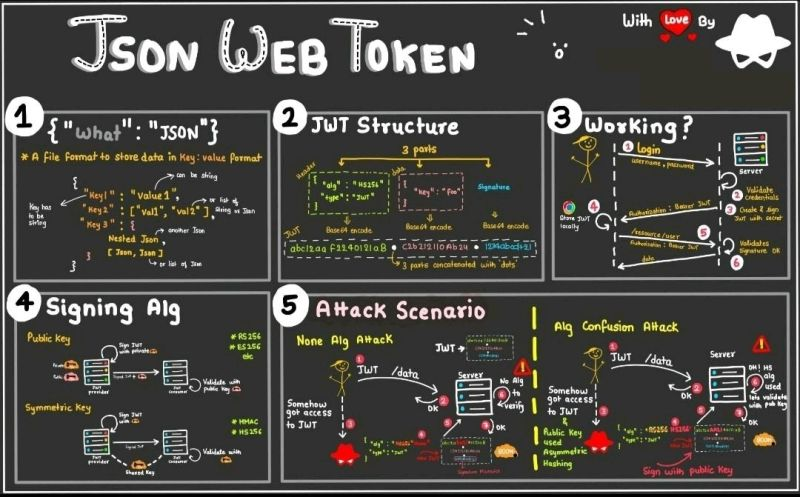
\includegraphics[width=.8\linewidth]{img/jwt.jpg}
                \caption{Použití JWT v~praxi}
                \label{model-jwt}
            \end{figure}

            \emph{JWT} sestává ze~tří částí, které jsou odděleny tečkou.
            
            \begin{enumerate}
                \item \textbf{Hlavička (header)}, která obsahuje informace o~typu tokenu a~typu šifrování podpisu.
                \item \textbf{Tělo tokenu (body)}, které obsahuje data, která chceme uchovat (\emph{payload}).
                \item \textbf{Podpis (signature)}, který zajišťuje kontrolu, že~token nebyl během cesty na~server změněn.
            \end{enumerate}

            Všechny tři~části jsou zakódovány pomocí metody \emph{Base64} a~odděleny tečkou. Výsledný token je~také textový řetězec, který je~možné přenášet v~hlavičce \emph{HTTP~požadavku}.

            Jednou z~výhod \emph{JWT} je~možnost přenositelnosti. Token může být~vytvořen na~jednom serveru a~ověřen na~jiném, který má k~dispozici daný klíč (\cite{ieee:jwt}). Můžeme tak např.~umožnit jednotné přihlášení v~rámci několika služeb. \emph{JWT}~není vázán na~symetrické šifrování a~tak se~k~využití přenositelnosti často využívá \emph{asymetrické šifrování}~--~n\,--\,tice klíčů, kde hlavní server má tzv.~\emph{privátní klíč} a~ostatní mají svůj~vlastní \emph{veřejný klíč}, odvozený od~privátního, kterým ověřují, že~byl~token vytvořen na~správném serveru. \cite{miguelgrinbergJSONTokens}.
            
            \emph{Veřejných klíčů} je~možné v~rámci \emph{asymetrického šifrování} vytvořit více a~přidělit je~různým službám, které je~pak mohou používat pro~ověření tokenu.

            Formát \emph{Base64} je~kódování, které používáme pro~jednodušší přenos dat, a~nikoliv pro~zabezpečení. Bezpečnost \emph{JWT} je~zajištěna pouze podpisem, který zaručuje \emph{integritu dat}. Data ale~může číst kdokoliv, kdo získá~přístup k~tokenu. Proto je~důležité do~tokenu ukládat pouze data, která jsou nezbytně nutná a~neobsahují citlivé informace. K~šifrování dat a~ostatních částí \emph{JWT} vznikly navazující standardy\,--\,\emph{JWE}, \emph{JWS}, \emph{JWA} a~\emph{JWK}. \cite{jwtesak}

            Zajímavou možností je~využití \emph{homeomorfního šifrování}, které umožňuje pomocí speciálního klíče provádět operace přímo nad~zašifrovanými daty, aniž bychom je~museli předem dešifrovat. \cite{graham2021ethical}

            \subsubsection{SQL Injection}
            \emph{SQL Injection} je~zřejmě nejčastější typ útoku, při~kterém útočník vloží kus \emph{SQL dotazu} (\emph{SQL Query}) do~neošetřeného uživatelského vstupu (např.\,vstupní pole pro~email) a~pokud jej~autor aplikace neošetří, je~místo zpracování vykonán společně se~zbytkem dotazu. To~může vést k~získání citlivých dat, jejich změně nebo~smazání. Může např.~dojít ke~změně hesla administrátorského účtu a~tím získání přístupu ke~chráněným datům.

            Proto je~nutné data od~uživatele vždy ošetřit a~v~ideálním případě použít navíc tzv.~\emph{Parametrizované dotazy} (\emph{Prepared statements}). Při~použití \emph{parametrizovaných dotazů} se~do~dotazu nevkládají přímo data, ale na~místo, kam~patří data je~vložený tzv.~\emph{Zástupný symbol} (\emph{placeholder}), který je~poté nahrazen ošetřenými (\emph{escapovanými}) daty tak, aby~nebylo možné případný vložený příkaz provést. Zástupný symbol v~SQL představuje otazník \uv{\texttt{?}} nebo v~případě pojmenovaných hodnot název proměnné za~dvojtečkou \uv{\texttt{:nazev}} \cite{graham2021ethical}
            
            Např.~dotaz na~změnu emailové adresy, který by~v~případě neošetření umožnil útočníkovi získat administrátorský přístup do~aplikace, by~mohl vypadat, jako v~ukázce \ref{model-sql-injection}.:
            \begin{figure}
                \begin{subfigure}{0.48\textwidth}
                    \centering
                    \begin{minted}{go}
id := 42
// nebezpečný vstup od uživatele
email := "mujmejl@seznam.cz', role='admin"
// příme spuštění dotazu
DB.Exec("UPDATE users SET email = '" + email + "' WHERE id = " + id)
                    \end{minted}
                    \begin{minted}{sql}
-- výsledný spuštěný dotaz, který by umožnil útočníkovi získat administrátorský přístup
UPDATE users SET email = 'mujmejl@seznam.cz', role='admin' WHERE id = 42
                    \end{minted}
                    \subcaption{Příklad útoku SQL Injection}
                \end{subfigure}
                \begin{subfigure}{0.48\textwidth}
                    \centering
                    \begin{minted}{go}
id := 42
// nebezpečný vstup od uživatele
email := "mujmejl@seznam.cz', role='admin"
// příprava dotazu pomocí "prepared statements"
DB.Exec("UPDATE users SET email = ? WHERE id = ?", email, id)
                    \end{minted}
                    \begin{minted}{sql}
-- ošetřený (escapovaný) dotaz, který by pouze vložil do databáze nevalidní emailovou adresu
UPDATE users SET email = 'mujmejl@seznam.cz\', role=\'admin', WHERE id = 42'
                    \end{minted}
                    \subcaption{Ošetření pomocí prepared statement}
                \end{subfigure}

                \caption{SQL injection a jeho ošetření}
                \label{model-sql-injection}
            \end{figure}

            Samozřejmě v~příkladu není vstup nijak ošetřen a~k~přijetí takové hodnoty do~pole \texttt{email} by~nemělo vůbec dojít, jelikož nejde o~validní emailovou adresu. Proto je~potřeba vstupní data v~aplikaci ošetřovat nejméně na~2~místech. Vstupní data a~parametrizované dotazy. Také je~dobré zavést kontrolu~před odesláním na~straně uživatele, nicméně na~to~nelze spoléhat, jelikož odeslání dat lze~jednoduše obcházet.
            
            Další kontroly vstupních dat mohou probíhat i~na~úrovni databáze. To~je ale už~na~uvážení autora aplikace. \cite{w3s:SQLInjection}, \cite{itnetwork:SQLInjection}

            \subsubsection{XSS~--~Cross Site Scripting}
            \emph{XSS} je~útok, při~kterém útočník vloží do~uživatelského vstupu kód, který se~při~načtení stránky spustí. To~může vést k~získání citlivých dat, přesměrování na~jinou stránku, nebo~k~jiným nežádoucím akcím.

            Jelikož v~projektu používám React, který využívá \emph{JSX}, je~tento typ útoku téměř vyloučen. \emph{JSX} totiž neumožňuje vkládat do~HTML kód, ale~pouze textové řetězce, které se~při~načtení stránky zobrazí.

            Existují ale výjimky, to~je~použití \texttt{eval}, která spouští Javascript kód v~řetězci, a~přímé vkládání neošetřeného vstupu pomocí \texttt{dangerouslySetInnerHTML} nebo jiných vlastností, které se přímo přepíšou do~kódu, např.~\texttt{href}, \texttt{OnClick}~apod.

            Možnou ochranou před tímto typem útoku je nahrazení znaků, které mohou způsobit problémy, za~jejich \emph{HTML entity}, kde je~potřeba znaky jako~\texttt{<} nahradit za~\texttt{\&lt;}, \texttt{>} za~\texttt{\&gt;}, \texttt{\&} za~\texttt{\&amp;}~apod.. Takové \emph{HTML entity} prohlížeč vykreslí uživateli a~nezpracovává je~jako~funkční kód.
            
            Možností je~také využít specializované knihovny, které toto ošetření provedou za~nás, a~nebudeme muset řešit, které znaky je~potřeba ošetřovat. Např.~\emph{DOMPurify} nebo \emph{sanitize-html}. \cite{medium:XSS}

        \subsection{Testování}
        Testování je~důležitou součástí vývoje aplikace a~černé svědomí velké části vývojářů. Testování je~časově náročné a~vývojáři se~mu~často vyhýbají, protože je~potřeba vytvořit sadu testů, které pokryjí všechny možné situace, které mohou nastat.
        
        Na~druhou stranu~--~zejména automatickým~--~testováním můžeme ušetřit spoustu času, který bychom jinak strávili ručním testováním aplikace nebo při hledání chyb, které se~objevily po~změnách v~kódu aplikace. Automatické testování umožňuje vytvořit sadu testů, které můžeme spustit při~každé změně aplikace a~ověřit si~tak, že~aplikace stále funguje správně.
        
        Např.~při~změnách základní funkcionality je~dobré otestovat, že~i~po~změnách fungují stále stejně. Zejména testujeme tzv.~\emph{čisté funkce}, což jsou funkce, které nemají žádné vedlejší efekty a~vždy vrací stejný výsledek pro~stejný vstup. Takové testování nazýváme \emph{unit testing}.
        
        V~každém jazyce existují nástroje pro~automatické testování. Např.~v~případě Javascriptu jsou~to~\emph{Jest}, \emph{Mocha}, \emph{Chai} nebo \emph{Jasmine}. Go~má~vestavěný nástroj pro~testování~\emph{Go~test}.
        
        Pro~testování React aplikace budu používat \emph{Jest}. Pro~testování backendu budu používat \emph{Go~test} \cite{jestjsTestingReact}.
        
        \subsubsection{Testování API}
        Pro~automatické testování API existují nástroje, které umožní vytvářet požadavky bez~nutnosti mít~hotovou \emph{frontendovou} část. Mezi nejznámější patří \emph{Postman}, \emph{Insomnia} nebo \emph{Swagger}. Některé navíc nabízejí možnost vytvořit si~sadu automatických testů, které můžeme automaticky spustit při~sestavení aplikace a~ověřit si~tak, že~API stále funguje správně.

        K~tomuto účelu využívám \emph{Postman}. S~nastaveným testovacím skriptem si~jednoduše ukládám nový \emph{token} a~při~dalším požadavku ho~posílám v~hlavičce požadavku. Tímto způsobem můžu testovat backend, bez vypínání bezpečnostních opatření.

        \subsubsection{Testování frontendu}
        Pro~testování frontendu budu používat knihovnu \emph{Jest}, kterou na~testování používá např.~Facebook. Testovat~bude potřeba čisté funkce, ale také komponenty. Komponenty se~testují pomocí snapshotů, které porovnávají vykreslenou komponentu s~předchozí verzí. Pokud se~liší, test selže a~je~potřeba zkontrolovat, zda~je~změna v~pořádku. \cite{jestjsTestingReact}

        \subsection{Údržba aplikace}
        Údržba aplikace je~důležitá část vývoje. Je~potřeba aplikaci pravidelně aktualizovat a~opravovat chyby, které se~vyskytnou.
        Tedy jde o nejdelší část životního cyklu aplikace. V~této části je~potřeba aplikaci testovat a~opravovat chyby, které se~vyskytnou.
            
            \subsubsection{SDLC~--~Životní cyklus vývoje software (Software Development Life Cycle)}
            SDLC je~životní cyklus vývoje softwaru. Jedná se~o~soubor procesů, které se~používají při~vývoji softwaru.
            Tyto procesy se~opakují v~kolech, které se~nazývají iterace. V~každé iteraci se~vyvíjí část aplikace, která je~následně testována.
            Vývojáři se~také mohou v~každé iteraci vrátit k~předchozí části a~upravit ji~podle potřeby.
            
            Existuje několik modelů \emph{SDLC}, které se~liší počtem iterací a~způsobem vývoje. Nejčastěji se~používá model \emph{Agile},
            který je~založen na~iteracích a~pravidelné komunikaci se~zákazníkem. V~každé iteraci se~vyvíjí část aplikace, která je~následně testována.
            
            Existují ale i~jiné modely vývoje, jako např.~\emph{Vodopádový}, který je~založen na~jedné iteraci.
            V~té se~vyvíjí celá aplikace a~až poté se~testuje a~nasazuje.
            V~případě chyby je~potřeba se~vrátit na~začátek a~vyvíjet aplikaci znovu.

            \subsubsection{Sledování chyb nahlášených uživateli}
            Pokud uživatel narazí na~chyby v~aplikaci, měl~by~je~mít~možnost nahlásit. Vývojář má~potom lepší možnost tyto chyby sledovat a~opravit~je.

            Podobný je~i~případ požadavků na~nové funkce. Uživatel by~měl mít~možnost požádat o~novou funkci nebo zlepšení stávajících,
            aby~vývojář mohl aplikaci dále rozvíjet.

            \subsubsection{Běhové a kompilační chyby}
            \emph{Kompilace} je~proces překladu zdrojového kódu do~binárního souboru, který je~přímo spustitelný na~procesoru. Při kompilaci se~kontroluje správnost kódu, datových typů ap. Případné chyby překladač oznámí vývojáři. Některé chyby může překladač opravit automaticky a~podle závažnosti chyby a~námi zavedených parametrů překlad proběhne v~pořádku nebo se~zastaví a~je~potřeba chyby nejdříve opravit.

            Chyby se~ale mohou projevit až~při~běhu programu. To~jsou chyby, které např.~závisí na~datech, která se~do~programu načítají. Příkladem takové chyby může být špatná práce s~pamětí, která může vést k~přetečení paměti a~následnému pádu programu.

            Na běhových chybách se~docela často zakládají útoky na~aplikace. Útočník může záměrně zasílat data, která způsobí chybu v~aplikaci, čímž může získat přístup k~systému nebo získat data, ke~kterým by~jinak přístup neměl.

            Důležité pro opravu chyb je~uvědomit si~jejich příčinu. To~je~často složité, protože chyba se~může projevit až~po~několika krocích nebo pouze za~specifického stavu aplikace.

            Proto je~nutné aplikaci testovat a~opravovat chyby, které se~vyskytnou. To~je~důležitá část vývoje aplikace. Důležité je~také sledovat chyby, které se~vyskytnou uživatelům. Jeden z~nástrojů, které to~umožňují, je~\emph{Sentry}.

            \subsubsection{Sentry}
            \emph{Sentry} je~nástroj, který umožňuje zachytávat chyby za~běhu aplikace. Pomocí webového rozhrání potom může vývojář (nebo jeho tým) sledovat chyby, které se~vyskytly za~chodu~aplikace. \emph{Sentry} umožňuje sledovat chyby v~různých jazycích, jako v~našem případě \emph{Javascript a Go}. Ale funguje i~v~dalších jazycích.


            V~každém z~těchto jazyků umožní \emph{Sentry} sledovat chyby specifické pro~daný jazyk a~tím zjednodušit opravu chyb. Např.~v~případě \emph{Javascriptu} umožní sledovat akce, které uživatel provedl, před tím, než došlo k~chybě. Chyby z~backendu i~frontendu aplikace se~uloží na~jedno místo a~je~tak jednodušší s~nimi pracovat.

            Díky tomu má~vývojář k~dispozici spoustu informací, které potřebuje k~nalezení, vyvolání a~opravě chyby. Sentry také umožňuje přímo vytvářet \emph{úkoly}, na kterých mohou vývojáři pracovat. To~umožňuje vývojářům efektivněji rozdělovat práci na~opravách chyb, které \emph{Sentry} zachytí.

            Informace navíc zůstanou uloženy v~\emph{Sentry} a vývojáři se~k~nim mohou kdykoliv vrátit. Sentry je možno integrovat do~různých komunikačních nástrojů, jako např.~Slack, který se~běžně používá ke~komunikaci ve~vývojových týmech a~upomínka na~chybu se~objeví přímo v~komunikačním kanálu týmu.
	
        \subsection{Verzovací systém GIT}
        \emph{GIT} vytvořil autor Linuxu \emph{Linus Torvalds} v~roce 2005. Je~to~distribuovaný verzovací systém. To znamená, že~každý vývojář má~lokální kopii celého projektu, tedy může pracovat i~bez~připojení k~internetu a~následně své~změny nahrát na~server, když se~připojí.
        
        Základní funkcí \emph{GITu} je~ukládání změn. Neukládáme celé soubory, ale pouze změny, které se~udály. Díky tomu je~možné spravovat i~velké projekty s~více vývojáři a~po~dokončení části práce vidět, co~který vývojář udělal a~spojit do~jednoho celku, na~kterém se~dále pracuje. Díky verzování je~také možné se~kdykoliv vrátit k~předchozí verzi projektu a~pokračovat ve~vývoji od~této verze nebo~pracovat na~několika různých verzích zároveň díky větvím. Výslednou práci můžeme označit pomocí tagů, které se~používají zejména pro~označení oficiálních vydání aplikace, nicméně je možné je~použít i~v~jiných významech.
        
        To~umožňuje vývojářům pracovat na~různých problémech projektu paralelně a~následně je~sloučit do~jednoho celku.

        Existují taky různé služby, které poskytují prostor pro~ukládání projektů online, tak~aby~byly zálohované a~přístupné odkudkoliv, jako např.~\emph{GitHub}, \emph{GitLab} nebo~\emph{Bitbucket}. Mimo zmíněné funkce nabízejí třeba možnost vytvářet \textbf{Issues}, které může vývojář vytvořit, pokud narazí na~chybu nebo~má~nápad na~vylepšení. Tímto způsobem může sdělit svůj nápad nebo~chybu v~aplikaci a~případně se~k~ní vrátit později. \emph{Issues} je~také možné přiřadit konkrétnímu vývojáři, který se~o~danou chybu nebo~nápad postará, a~automaticky vytvořit větev, na~které bude práce probíhat. Na konci práce vývojář vytvoří tzv.~\textbf{Merge Request}, kde oznámi, jak problém řešil, a požádá o~sloučení nového kódu do~hlavní větve projektu. Je~taky možné jednoduše zobrazit rozdíly mezi hlavní větví a~tou, na~které vývojář pracuje.
        
        \emph{GIT} je~pro~vývoj dnešních aplikací nepostradatelný nástroj. \cite{gitscmBook}
        
        \emph{Gitlab} je open-source nástroj pro~správu verzí na~serveru. Nabízí také možnost vytvářet \emph{Issues}, \emph{Merge Requesty} a~další funkce. Je~možné jej~nainstalovat na~vlastní server a~mít~tak~plnou kontrolu nad~svými daty, což~využívá spousta společností, které mají např.~více projektů.

        \subsection{Linux a příkazová řádka, WSL2}
        Linux je~operační systém, který vytvořil Linus Torvalds v~roce 1991. Je~to~nejrozšířenější open source operační systém, používaný zejména na~serverech ale také na~\emph{desktopových zařízeních} v~podobě mnoha distribucí.
        
        Je~to~také základ pro~mnoho dalších operačních systémů, jako např.~\emph{Android open--source project (\emph{AOSP})} od~společnosti \emph{Google}, který na~\emph{jádro OS Linux} přidává funkce pro~použití na~mobilních zařízeních. \cite{AOSP:linux}
        
        Velikou výhodou je otevřenost a~možnost upravovat zdrojový kód. To~umožňuje vývojářům upravovat systém podle svých potřeb. Výhodou je~také jeho bezpečnost a~svoboda. V~porovnání s~jinými operačními systémy je~mnohem bezpečnější a~méně náchylný k~virům. \cite{medium:LinuxSecure}

        Nabízí mnoho grafických prostředí, takže si~uživatel může vybrat, jakým způsobem bude systém používat a je možné téměř
        všechno nastavit tak, jak v práci potřebuje. Navíc většina nástrojů pro vývoj webových aplikací je~vyvíjena pro~Linux, takže je~možné je~používat bez~problémů a~automaticky vše nastavit skriptem z~příkazové řádky. Není nutné instalovat a~mít~spuštěno 5 různých nástrojových oken, vše je~na~jednom místě.

        Na~Windows je~možné Linux využívat pomocí \emph{WSL2 (Windows Subsystem for Linux)}. Jedná se~o~virtuální stroj, který běží na~pozadí a umožní uživateli Windows používat výhody, které nabízí Linux, např.~má~vývojové nástroje na~jednom místě, místo několika oken, které musí mít~otevřené při~normálním vývoji na~Windows.

        \subsection{IDE a nástroje pro psaní kódu}
        \emph{IDE} (Integrated Development Environment) je~integrované vývojové prostředí, které umožňuje vývojářům psát kód, spouštět aplikaci a~ladit (debugovat) ji~v~jednom prostředí. To~umožňuje vývojářům pracovat efektivněji a~rychleji. V~jednom editoru mají~všechny nástroje, které potřebují k~vývoji aplikace. V~dnešní době existuje spousta IDE, které se~liší podporovanými jazyky, funkcemi a~vzhledem. Funkcionalitu je~možné doplňovat o~nové funkce pomocí pluginů.
        
        Mezi nejznámější \emph{IDE} patří \emph{Visual Studio Code}, \emph{IntelliJ IDEA}, \emph{Google Atom}, \emph{Netbeans} nebo \emph{Sublime Text}. Jako \emph{IDE} můžeme při~vhodném nastavení označit také konzolový editor \emph{Vim}.
        
        Důležitými funkcemi jsou zvýrazňování syntaxe, automatické formátování kódu, možnost spouštět aplikaci přímo z~\emph{IDE}, odchytávat a~ladit ji~v~něm. \cite{IDE}
        
        S~pokrokem \emph{umělé inteligence} (\emph{AI}) se~objevují nástroje, které dokáží automaticky opravovat chyby v~kódu, nebo~dokonce přímo psát kód za~vývojáře. To~ale zatím není možné v~každém jazyce a~funguje to~pouze pro~jednoduché úlohy. Navíc je~nutné kód osobně zkontrolovat, protože nástroje mohou vytvořit kód, který je~sice funkční, ale~neefektivní nebo~nečitelný.

        Příkladem nástroje generování kódu může být~např.~\emph{Github Copilot}, který dokáže na~základě komentářů nebo kontextu v~kódu vygenerovat funkční pokračování kódu. Další nástroje jsou \emph{Tabnine}, \emph{Kite} nebo \emph{Deep TabNine}. \cite{sz:AI}
        
        V~průzkumu \uv{The State Of AI Tools 2023}~(\cite{zerotomasteryStateOfAI}) většina vývojářů odpověděla, že~se~nebojí toho, že by~je~\emph{AI} v~blízké budoucnosti plně nahradila. Programování je~komplexní proces, který vyžaduje kreativitu a~schopnost řešit problémy různého typu. Využití kódu od~\emph{AI} je~nutné brát s~rezervou~--~učí se~z~kódu, co~vytvořili lidi, takže může být~ovlivněný chybami a~nedostatky a~prozatím není~schopná samostatně přemýšlet nad~řešením problému, ale~pouze generovat kód na~základě předchozích řešení, která mohou být chybná či~neefektivní.
        
        Jazykové modely \emph{AI}, jako např.~\emph{ChatGPT} potom pomáhají zejména ke~konzultaci problémů a~získání nápadů, jak je~vyřešit. Svým způsobem tím~nahrazují \emph{Stack Overflow}~--~síť, kde~si vývojáři navzájem radí s~řešením problémů, zejména z~oboru~\emph{IT}. Tyto pomocné nástroje jsou také skvělé na~opakované úkoly, jako přepisování struktur dat nebo hromadných příkazů.

        \emph{AI} nástroje typu \emph{ChatGPT} ale poslední dobou ztrácí na~přesnosti. Je~to~díky tomu, že~k~dalšímu učení využívají data přístupná z~internetu, a~to~často i~data generovaná jinými \emph{AI} systémy. Výsledky je~tedy nutné posuzovat kriticky. \cite{computerworld:AI}

	\section{Návrh aplikace}
        Před samotným vývojem aplikace je~potřeba se~zamyslet, jak bude aplikace fungovat, jaké bude mít funkce a~jak bude vypadat. Tvoříme tzv.~\emph{funkční požadavky} na~výslednou aplikaci. Potom můžeme vytvořit \emph{UML modely}, které mohou pomoct blíže si~promyslet strukturu a~uvědomit si~některé další aspekty vývoje, které nás~mohou potkat.

        Na~začátku plánování projektu je~dobré se~zamyslet i~nad~tím, jaké technologie budeme používat, jak budou jednotlivé součásti komunikovat a~jakým způsobem budeme aplikaci vyvíjet \cite{bctynovsky:specifikacepozadavku}. V~profesionálním prostředí je~potom důležité přemýšlet i~nad~tím, jestli budeme aplikaci vyvíjet sami nebo~v~týmu a~zda je~na~trhu práce dostatek lidí, kteří dané technologie znají.

        \subsection{Účel a~popis fungování vyvíjené aplikace}
        Aplikace \emph{Písemkomat}, poskytne registrovaným uživatelům možnost vytvořit vytvořit si příklady, umístěné ve~volitelně strukturovaných kategorií~--~podle předmětu, ročníku, tématu... Tyto příklady bude možné následně využít při tvorbě testů, kde~bude mít~uživatel možnost zvolit kategorie, ze~kterých se~vybere určené množství příkladů, nebo konkrétní příklady, které se~mají do~testu vložit. Uživatelé budou mít možnost přihlášení pomocí více způsobů, vč.~externích poskytovatelů ověření identity a~samozřejmě také pomocí přihlašovacího jména a~hesla.
        
        Řekněme, že~uživatel bude chtít pro~své žáky vytvořit několik verzí testu s~rozdílným zadáním příkladů. Zaregistruje~se do~aplikace, ověří svoji mailovou adresu a~přihlásí se~do~svého účtu. Jde~o~učitele matematiky, takže si~vytvoří 5~příkladů z~tohoto předmětu a~vloží je~do~kategorie \emph{Matematika} a~podkategorie \emph{Lineární rovnice}.

        Následně si~vytvoří test a~může si~vybrat, zda~chce, aby~se~v~jeho testu objevily všechny příklady z~dané kategorie nebo zkombinovat příklady z~růzých kategorií. Nakonec otázky v~testu chce~nechat náhodně seřadit. Příklady jsou navíc zapsány obecně pomocí proměnných, takže v~každé verzi budou příklady s~náhodně dosazenými hodnotami. Jelikož některé hodnoty nemohou být~zcela náhodné, jinak by~to mohlo vést ke~složitě řešitelným nebo pro~danou úroveň zcela neřešitelným příkladům, bude možné vytvářet mezivýpočty v~rámci proměnných. Aplikace umožní vytvořit si~proměnné, které budou mít~přiřazenou náhodnou hodnotu z~určitého intervalu nebo vypočtené z~jiných proměnných.

        Uživatel si~vytvoří proměnné $A, B, C$ a $D$, kde $A, B$ definuje jako náhodná \emph{lichá} čísla od~1 do~10, $C = 4/3*A$ a $D = C + B$. Řešený příklad se~vygeneruje podle předlohy, kterou si~uživatel vytvořil. Do~proměnných $A, B$ se~při~konečném generování příkladů uloží náhodné číslo z~intervalu, který~si~uživatel nastavil a~pomocí zápisu proměnné \texttt{\$\{A\}} se~vloží do~příkladu či~proměnných na~zadané místo. Proměnné budou vyčísleny, nebo zachovány jako původní nezpracovaný text. Funkční proměnné budou moci kromě generování čísel obsahovat také vstupní pole, jako např. výběr z~možností, nebo textové pole, které bude mít~za~úkol žák vyplnit. Při~generování se~proměnné doplní do~zadání, případně do~možností výběru, pokud je~uživatel nastaví. V~případě, že~zadá vzorec, ze~kterého bude možné možnosti vygenerovat, bude možné určit, kolik odpovědí chce~generovat. Aplikace pohlídá, že~uživatel označí alespoň jedno správné řešení. Příklady bude možné komentovat a~hodnotit, aby bylo jednodušší najít chyby v~zadání.
        
        Předpokládejme, že~budou vygenerována náhodná čísla $A = 3$ a~$B = 5$ a~hodnoty proměnných $C, D$ jsou~zadány takto:
        \begin{align*}
            \$A &= 3 \\
            \$B &= 5 \\
            \$C &= 4/3*\$A = 4/3*3 = 4 \\
            \$D &= \$C + \$B = 4 + 5 = 9
        \end{align*}

        Proměnné se~při~generování výsledné podoby příkladu nahradí vygenerovanými čísly, výrazy nebo funkčními prvky. Po vygenerování příkladu bude potřeba uložit do~databáze konkrétní vygenerované hodnoty proměnných a~možností odpovědí, aby bylo možné identifikovat přesnou verzi příkladu. Pokud se~v~příkladě nevyskytují žádné proměnné nebo není potřeba nic generovat, potom není potřeba hodnoty ukládát.

        Proměnné bude možné shlukovat do~variant. To~umožní vytvořit více variant příkladů. Např.~varianta, kde~se~budou generovat čísla celá a~varianta, kde~se~budou vyskytovat i~zlomky. Učitel si~pak~při~tvorbě testu jen vybere, kterou variantu chce použít.

        Učitel bude také mít~možnost zvolit~si, jestli chce~vytvořit otevřenou nebo uzavřenou formu příkladu s~možnostmi výběru. V~tomto případě může taky využít proměnné, které si~vytvořil dříve. V~obou případech může taky zapsat vzorec, ze~kterého se~vypočtou možnosti a~označit správnou možnost. Pokud učitel pro tvorbu možnosti využije vzorec, bude možné jich z~jedné možnosti vytvořit několik. Ve~výsledném příkladu se~v~možnostech výběru proměnné nahradí a~výraz se~vyčíslí, pokud nebude přepínači určeno jinak.

        Výsledná podoba vzoru příkladu jednoduchého výrazu může vypadat např.~takto:
        \begin{align*}
            \text{Vyřeš v oboru N:} \quad \$Ax + \$B &= \$C + \$D \\
            \begin{aligned}
                a) \quad &\text{Nemá řešení v oboru N} \\
                b) \quad &\text{x = \$A} \\
                c) \quad &\text{x = \$B} \\
                d) \quad &\text{x = \$\{\$A * \$B - 2\}} \\
            \end{aligned}
        \end{align*}

        Po~vygenerování a~dosazení hodnot:
        \begin{align*}
            \text{Vyřeš v oboru N:} \quad 3x + 5 = 4 + 9 \\
            \begin{aligned}
                a) \quad &\text{Nemá řešení v oboru N} \\
                b) \quad &\text{x = 3} \\
                c) \quad &\text{x = 5} \\
                d) \quad &\text{x = 13} \\
            \end{aligned}
        \end{align*}

        Vstupní políčka se~ve~výsledné práci vykreslí jako prázdné nebo podtržené místo o~velikosti určené při~zadávání proměnné. V~případě otázky s~možnostmi výběru se~na~místě vykreslí všechny možnosti, aby~žák mohl vybrat správnou možnost kroužkováním nebo jinak, jak učitel určí.
        
        To umožní systém používat např.~pro jazykové předměty, kde student doplňuje slova do~textu nebo~výbírá vhodné písmeno.

        Některá nastavení bude možné ovlivnit (měnit velikosti, počty možností, vybrat šablonu, zapnout/vypnout náhodné řazení otázek nebo odpovědí) i~na úrovni celých testů. Pokročilý uživatel potom bude mít možnost vytvořit si~vlastní šablony pro výpis příkladu.

        \subsection{UML~--~Unified Modeling Language}
        Jeden ze~standardních nástrojů pro~modelování aplikace je~\emph{UML}. \emph{UML} je~standardizovaný grafický jazyk pro~modelování softwarových systémů. První verze byla vydána v~roce 1997 a~od~té~doby se~stala standardem pro~modelování softwarových systémů. Základem \emph{UML} je~\emph{UML diagram}, který slouží k~vizualizaci návrhu aplikace. \cite{uml:diagram}
        
        Specifikace definuje základní dva typy diagramů:
        \begin{itemize}
            \item \textbf{Strukturální diagramy} popisují strukturu systému, tedy jeho části a~vztahy mezi nimi. Může jít např.~o~diagramy tříd, objektů, komponent, nebo~komunikace mezi~komponentami\dots
            \item \textbf{Diagramy chování} popisují chování systému, tedy jak se~jeho části chovají a~jak spolu komunikují. Např.~diagramy aktivit, stavový diagram, nebo~diagram případů užití\dots
        \end{itemize}

        Pro naplánování své práce jsem si~vybral diagramy ze~standardu \emph{UML}\,--\,\textbf{diagram případů užití} \textbf{Use Case Diagram} a~\textbf{diagram~tříd} \textbf{Class Diagram}. Diagramy budu~zpracovávat pomocí nástroje \emph{Creately}, což je~webová aplikace, umožňující jednoduchou úpravu diagramů. Diagramy je~možné tvořit i~v~jiných aplikacích, např.~\emph{Draw.io}~ap. Je důležité zmínit, že neexistují předem dané postupy, jak diagramy tvořit. Způsob, jakým vývojář funkcionalitu modeluje je~čistě na~jeho osobním zvážení, dokud se~drží definice \emph{UML}. Je~ale důležité, aby svá~rozhodnutí vývojář zdůvodnil a~průběžně dokumentoval. \cite{uml:diagram}

        \subsubsection{UCD~--~Use Case Diagram}
        \emph{UCD} je~diagram ze~standardu \emph{UML}, který popisuje chování systému z~pohledu uživatele, tedy interakci systému s~uživatelem. Jednotlivým aktérům jsou přiřazeny případy užití, které popisují, jaké akce mohou jednotliví aktéři používat.

        To~umožní lépe si~představit, jak bude aplikace fungovat, jaké funkce bude mít a~jaké \emph{endpointy} budeme potřebovat vytvořit, aby~bylo možné akce provést. Taky si~můžeme ověřit správnost návrhu a~zjistit, zda~jsme nějakou funkcionalitu nevynechali, protože na~diagramu jsou případné nedostatky vidět lépe. Tvorba \emph{UCD} vychází ze~specifikace funkčních požadavků aplikace. \cite{uml:usecase}

        Při~modelování pomocí \emph{UCD} se~používají symboly, které znázorňují jednotlivé části diagramu.
        \begin{itemize}
            \item \textbf{Aktér} je~osoba nebo systém, který používá aplikaci. Aktérem může být např.~uživatel, čas nebo~jiná aplikace. K~označení se~používají ikony lidí a~textový popisek.
            \item \textbf{Případ užití} je~akce, kterou aplikace \emph{aktérovi} nabízí. Případ užití je~zobrazen jako elipsa, která je~připojena k~aktérovi čarou.
            \item \textbf{Vztahy mezi~aktéry a~případy užití} znázorňují, jestli a~jakým způsobem může aktér případ užití používat. Vztahy se~značí šipkami, které vycházejí z~aktéra a~končí u~případu užití.
            \item \textbf{Rozšíření} (extend)~--~je~případ užití, který přejímá vlastnosti předchozího případu užití a~rozšiřuje je~o~další možnosti. Znázorňuje se~jako šipka, která míří směrem z~případu užití a~končí u~případu užití, který rozšiřuje.
            \item \textbf{Zahrnutí} (include)- zahrnutí je~případ užití, který je~součástí jiného případu užití. Znázorňuje se~jako šipka, která vychází z~případu užití, který zahrnuje a~končí u~případu užití, který je~zahrnut.
        \end{itemize}

        \subsubsection{Class Diagram}
        \emph{Class diagram} (\emph{Diagram tříd}) je~také součástí~standardu \emph{UML}. Zobrazuje třídy, jejich atributy a~metody a~vztahy mezi~nimi. Souvisí s~návrhem struktur uložených v~databázi a~modelů dat, se kterými pracuji v~aplikaci.

        \emph{Vlastnost (atribut)} třídy je~proměnná, která je~přiřazena k~třídě. Nese vlastnost, která dává~v~kontextu třídy smysl. Např.~třída \texttt{Auto} může mít~vlastnost \texttt{barva}, která bude mít~hodnotu \texttt{červená} a~vlastnost \texttt{maxSpeed}, která bude mít~hodnotu \texttt{200 km/h}.

        \emph{Metoda} třídy je~funkce, která je~přiřazena k~třídě. Může mít~parametry a~výstupní hodnotu. Např.~třída \texttt{Auto} může mít~metodu \texttt{drive}, která bude mít~parametr \texttt{speed} k~určení, jakou rychlostí má~auto jet.
        
        Třída je v~diagramu~tříd zobrazena jako obdélník rozdělený na tři části. V~první části je~název třídy, ve~druhé jsou vlastnosti a~ve~třetí metody. \emph{Veřejné} vlastnosti a~metody mají na~začátku názvu \texttt{+}, \emph{chráněné} \texttt{\#}, \emph{privátní} \texttt{-} a~\emph{statické} \texttt{\_}.
        
        \emph{Veřejné (public)} vlastnosti a~metody jsou přístupné ostatním třídám a~komukoliv, kdo~má~přístup k~objektu je~může zobrazit či~změnit. Vlastnosti a~metody mají na~začátku názvu \texttt{+}.

        \emph{Chráněné (protected)} vlastnosti a~metody jsou přístupné jen třídám, které dědí vlastnosti z~třídy, ze~které dědí. Na~začátku názvu píšeme~\texttt{\#}.
        
        \emph{Privátní (private)} vlastnosti a~metody jsou přístupné jen třídě, ve~které jsou definovány a~nikdo jiný s~nimi nemůže pracovat. Na~začátku názvu píšeme~\texttt{-}.
        
        \emph{Statické (static)} jsou vlastnosti a~metody, které jsou společné pro~všechny instance třídy a~tedy nejsou přidružené žádnému objektu a~lze~je~používat i~bez inicializace objektu. Označujeme znakem \texttt{\textunderscore}.
        
        Vztahy inkluze a~rozšíření jsou v diagramu tříd zobrazeny stejně jako u~\emph{UCD}.

        \emph{Diagram tříd} přímo souvisí s~návrhem struktur a~dat uložených v databázi. Lépe si~uvědomíme, jaká data bude nutné uchovávat v~databázi a~jaká jsou dočasná, nebo tyto~závěry můžeme z~diagramu jednodušeji vyvodit.

        Je také důležité udržovat \emph{diagram tříd} aktuální, protože se~může stát, že~se~v~průběhu vývoje změní návrh a~diagram tříd už nebude odpovídat aktuálnímu stavu aplikace. \cite{visualparadigmClassDiagram}.

        \subsection{Návrh struktury databáze}
        Pro~ukládání dat v~aplikaci použijeme databázi. Databáze je~soubor dat, která jsou~uspořádána tak, aby~byla snadno vyhledatelná a~měla nějaký význam.

        Při~plánování databáze využiju \emph{diagram tříd} k~plánování konkrétních tabulek a~vztahů mezi~nimi. \emph{UCD} pomůže zjistit, jaké SQL~dotazy nejspíše budou potřeba, což~umožní lepší náhled, které sloupce budou zařazeny do~indexů.

        O~problematiku tvorby databázových tabulek se~postará \emph{ORM} (\emph{Object-relational mapping}), který umožní vytvořit tabulky z~modelů dat, které budou používat aplikace. Autor aplikace se~tak nemusí starat o~tvorbu tabulek a~jejich vztahů, ale~může se~soustředit na~tvorbu aplikace, nicméně by~měl pamatovat na~zásady indexování a~optimalizace databáze. Tyto zásady jsou popsány jako 1\,--\,3.~normální formy a~do zásad \emph{ACID} (Atomicity, Consistency, Isolation, Durability). \cite{interval:normalniformydb, bmcACIDExplained}

        Potom následuje vytvoření tabulek, resp.~\emph{modelů dat}. Používá se~k~tomu jazyk \emph{SQL} (Structured Query Language), který bude ovládat databázi \emph{MySQL} (\emph{MariaDB}). Veškerou komunikaci prostřednictvím \emph{SQL} obstará \emph{ORM} systém.

        \textbf{Indexace} sloupců znamená optimalizaci dat v~daném sloupci pro~rychlejší třídění, spojování tabulek a~vyhledávání v~nich. \emph{Indexy} se~vytváří na~sloupcích představujících \emph{primární klíč} nebo \emph{unikátní} hodnoty, které se~v~tabulce nesmí vyskytnout opakovaně a~slouží k~jednoznačné identifikaci záznamu, nebo sloupců, které jsou~v~\emph{SQL} dotazech často využívány k~třídění a~vyhledávání. \emph{Indexy} je~možné připodobnit k~lékařské kartotéce, kde~se~snažíme, aby~karty pacientů byly~seřazeny abecedně, zdravotní sestra pak~při vyhledávání pacientů aplikuje metodu \textbf{binárního vyhledávání}, čímž~najde kartu dříve než~kdyby karty nebyly seřazeny. \cite{interval:normalniformydb, laurencik2018sql}

        \subsection{I18C~--~Mezinárodní lokalizace}
        \emph{I18C} je~proces přizpůsobení aplikace pro~daný jazyk a~kulturu, kromě překladu např.~formát data, měny nebo jednotky. Standard \emph{I18C} zahrnuje i~různé formy slov, např.~pro~různá množství. \cite{w3Internationalization}

        Každý znak je~v~počítači reprezentován číslem. V~minulosti používaly počítače k~ukládání znaků kódování \emph{ASCII}, které obsahovalo pouze 128 znaků (7 bitů, tj.~$2^7$, 0\,--\,127). To~znamená, že~bylo možné zobrazit pouze anglické texty a~některé interpunkční znaménka. 
        
        V~dnešní době se~většinově používá kódování Unicode (UTF), které k~původním 7~bitům (\emph{ASCII}) přidává nový význam prvnímu bitu, který má~význam, zda je~daný znak reprezentován více než~jedním bajtem. To~umožňuje zobrazit mnohem více znaků, vč.~např.~čínských znaků nebo~smajlíků, a tedy překlad aplikace do~různých jazyků a~znakových sad. Na~druhou stranu každý další byte znamená více použité paměti, kterou text zabírá a~počítač potřebuje více času na~zpracování každého znaku.
        
        Proto je~vhodné všechny~zdrojové kódy a~aplikace psát v~Anglickém jazyce, který využívá základní \emph{ASCII} znaky, a~aplikaci pro~uživatele překládat (\emph{lokalizovat}). Anglický jazyk je~navíc považován za~mezinárodní jazyk, který je~známý většině uživatelů a~aplikaci tak~jednodušeji zpřístupníme širší skupině uživatelů.
        
        Webový prohlížeč si~pamatuje preferenci jazyka uživatele a~při~požadavku na~aplikaci, zašle i~informaci o~preferovaném jazyce.

        Pro překlad aplikace se~používají \emph{lokalizační soubory}, které obsahují překlady jednotlivých textů aplikace. Každý jazyk má~svůj soubor, který se~načítá při~spouštění aplikace. Pokud překlad není nalezen, použije se~původní text.

        V~rámci \emph{backendu} aplikace je~potřeba přeložit zejména e-mailové zprávy a~hlášky, které budou odesílány uživatelům. V~rámci \emph{frontendu} pak~\emph{uživatelské rozhrání (UI)}, které bude používat uživatel.

        \subsection{Výběr technologií}
            Výběr technologií je~důležitý krok. Je nutné vybírat efektivní technologie, které budou dostatečně výkonné a~zároveň budou
            přívětivé pro vývojáře, aby vývoj nebyl zbytečně časově náročný. Je~dobré také myslet na~budoucí podporu a~rozšiřitelnost aplikace.

            \emph{React} použiju pro tvorbu \emph{Frontendu}. Umožní mi efektivní tvorbu uživatelského rozhrání, (\emph{User Interface, UI}).

            \emph{Typescript} samozřejmě použijeme i~při vývoji aplikace v~Reactu. \emph{Facebook} s~tím~samozřejmě počítá a~vydává
            kromě Reactu také balíček s~příslušnými datovými typy, pro použití v~Typescriptu. Typescript podporuje i~použití JSX šablon. \cite[Refeerence/Handbook/JSX]{TypeScript}

            \LaTeX je~profesionální nástroj pro~sazbu textů s~možnostmi matematických vzorců, který je~používán zejména v~akademickém prostředí.\cite{Rybicka2003:latex}
            
            \emph{MathJax} je~knihovna, která umožňuje zobrazovat matematické vzorce na~webových stránkách. Přijímá formáty matematiky zapsané ve~formátu, který používá systém \LaTeX. Ten~se poté převádí do~vizuální podoby, sestavené z~HTML prvků, kterou může prohlížeč zobrazit. MathJax nabízí i~možnost zobrazení ve~formě vektorové grafiky ve~formátu SVG. Díky tomu můžeme v~aplikaci názorně vykreslovat matematické vzorce, které se~vyskytnou v~příkladech nebo~učebních materiálech.\cite{abclinuxuMatematickxE9Vzorce}

            \emph{Go} je~staticky typovaný, kompilovaný jazyk vyvinutý společností Google v~roce 2007. Je to~jazyk, který je~velice rychlý a~jednoduchý na~psaní. Protože jde~o~kompilovaný jazyk, výsledný program~je~rychlý a~efektivní. Zároveň během vývoje není třeba celý program kompilovat, stačí jej~spustit příkazem \texttt{go run} a~aplikace funguje. Při~publikaci programu stačí spustit \texttt{go build} a~\emph{Go} vytvoří optimalizovaný spustitelný binární soubor. Je~to~jazyk, který je~velice oblíbený pro~tvorbu webových aplikací. Umožňuje při~vývoji jednoduše importovat existující balíčky z~GIT repozitářů, nebo jiných zdrojů přímo z~internetu, a~používat je~v~aplikaci a~sám si~tyto balíčky stáhne a~nainstaluje. Tím~značně urychluje vývoj aplikace.

            Zároveň při kompilaci vzniká jeden binární soubor, takže přestože je aplikace docela rozsáhlá, je~dostatečně rychlá.

            Základní funkce webových frameworků obecně je~tzv.~\emph{Router}, který umožňuje definovat jednotlivé \emph{koncové body} (\emph{endpointy}) a~typy požadavků, které můžeme využít pro~komunikaci s~nimi.
            
            Když~do~aplikace přijde požadavek, \emph{Router} zkontroluje, zda~existuje \emph{koncový bod}, který odpovídá požadavku a~pokud ano, předá požadavek příslušné \emph{Obslužné rutině} (\emph{handler}u).

            Každý \emph{koncový bod} má~svou~vlastní \emph{Obslužnou rutinu} (dále \emph{handler}), která zpracuje požadavek a~vrátí odpověď.
            Gin také umožňuje vytvářet skupiny \emph{koncových bodů}, které mají společný základ~URL adresy a které mohou mít společný \emph{handler}.
            To~umožňuje vytvářet aplikace, které mají jednotnou strukturu a~jsou přehledné. Např.~všechny \emph{koncové body} pro~přihlášené
            uživatele můžeme předem definovat a~zabezpečit.
            
            \emph{MySQL} je~relační databáze, která je~dnes jednou z~nejpoužívanějších databází. Je~dostatečně rychlá a~spolehlivá. \cite{databases21}
            MySQL~je~\emph{relační databáze}. Ukládá data v~databázích a~tabulkách, kde~jednotlivé sloupce určují typ dat a~jejich název. Každý řádek je~záznamem v~dané tabulce.
            
            Jednotlivé databáze~--~někdy používáme název \emph{schéma}~--~fyzicky na~disku reprezentují adresáře s~názvem konkrétní databáze. Jednotlivé~tabulky potom tvoří binární soubory s~příponou podle databázového \emph{enginu}, který používáme. V~našem případě používáme \emph{InnoDB}, který ukládá strukturu a~data v~souborech \emph{*.ibd}. \cite{MySQLInnoDB}
            
            \emph{GORM} je~ORM (ORM~--~Object-relational mapper) pro~jazyk Go. \emph{ORM} systémy umožňují jednoduše vytvářet databázové modely z~definovaných struktur. Z~nich \emph{ORM}~automaticky vytvoří všechny databázové tabulky, včetně těch relačních, a~při jakékoliv změně struktur také~automaticky změní tabulky v~databázi, v~rámci \emph{migrace modelů}. Struktury zároveň umožňují jednodušší kontrolu nad~daty, která se~do~databáze ukládají a~zjednodušují nám načítání konkrétních dat.

            Pokud je~potřeba nějaké složitější operace, samozřejmě je~možné využít i~samostatně formulované SQL dotazy. \cite{gormGORM, freecodecamp:orm}

            \emph{Vite} je~nový nástroj pro~vytváření \emph{Frontendu}. Je~to~nástroj, který je~velice rychlý a~jednoduchý na~použití.

            \emph{Docker, docker-compose} jsou nástroje, které umožňují vytvářet kontejnery, ve~kterých můžeme spouštět aplikace. Použití kontejnerů při~vývoji je~výhodné zejména při~spolupráci v~týmu, protože vždy když si~projekt znovu stáhneme a~spustíme, máme jistotu, že~aplikace běží v~na~aplikaci přizpůsobeném prostředí. To~umožňuje jednodušší zapojení dalších lidí do~vývoje a~nasazení aplikace na~různých platformách (např~.\emph{Windows}, \emph{Linux} i~\emph{MacOS}).

            Díky tomu~lze~rychle vytvořit kontejnery s~potřebnými službami, jako třeba databázi, na~jakékoliv platformě. Navíc je~kontejner přístupný pouze použitím specifického portu, čímž se~snižuje riziko útoku na~server, na~kterém aplikace běží. Na~jednom serveru je~tím~navíc umožněno provozovat více \emph{kontejnerů} (resp.~aplikací), dostupných na~různých portech. \cite{docker}

            \emph{Docker} resp. \emph{Docker-compose} bude v~mém projektu spravovat kontejnery s~aplikací (Vite~i~Go) a~databází kromě těch, které jsou potřeba pro chod aplikace.

            \emph{Nginx} se~sám~definuje jako webový server a~reverzní proxy server a~load balancer.

            Jako \emph{reverzní server} umožňuje přesměrovat požadavky na~různé servery, resp.~aplikace (porty), podle zadaných pravidel. Třeba podle URL adresy, typu požadovaného souboru nebo typu požadavku.
            
            \emph{Load balancer} zajišťuje rozložení zátěže mezi servery (resp.~více instancemi aplikace), které má~k~dispozici. To~se~využívá u~větších aplikací, které mají vysokou používanost nebo v~případě že~jednotlivé součásti aplikace běží na~více serverech nebo využívá externí služby. Taky je~možné nastavení záložních serverů pro~případ, že~nastane výpadek nebo přetížení hlavního serveru.
            
            \emph{Nginx} je~ve~srovnání s~jinými servery, jako např.~Apache, považován za~velmi rychlý. Zejména pak~při~obsluze požadavků na~statické soubory. Je~napsán v~jazyce C a~je~dostupný pro~většinu operačních systémů. \cite{WhatNGINX}

            A~\emph{Alpine Linux} je~odlehčená distribuce Linuxu, která je~určena zejména pro~nasazení v~kontejnerech, kde~očekáváme malou zátěž na~uložiště a~zdroje, nicméně jde~o~plnohodnotný systém a~je~možné jej~jako hlavní systém použít. Celková velikost distribuce po~instalaci je~pouze 5~MB, což je~velice málo.

            Tuto distribuci používám jako hlavní systém na~svém VPS\footnote{VPS~--~Virtual Private Server}, kde~aplikace poběží. Na~serveru poběží pouze \emph{Nginx}, který nasměruje požadavky na~správné porty, a~\emph{Firewall} (\texttt{UFW}), který zablokuje přístup k~portům, které nechci vystavovat na~veřejnost.

            Kombinací těchto technologií bych rád dosáhnul co~možná~nejlepšího poměru výkonu a~bezpečnosti.
	
	\section{Postup implementace}
        Nejprve je~potřeba vytvořit základní strukturu aplikace. Rozhodl jsem~se, že~pro lepší automatizaci budou vývojové i~produkční prostředí tvořit \emph{Docker kontejnery}, což~zajistí konzistentní prostředí pro~vývoj i~produkci, kdekoliv aplikaci spustíme.
        
        \textbf{Vývojová verze} bude obsahovat kontejnery pro~React, Go a~databázi. \emph{Go}~kontejner bude obsahovat nástroj \emph{Air}, který umožní automatický restart aplikace při~změně kódu \emph{backendu}. Při~vývojí ve~\emph{Vite} využijeme přesměrování (\emph{proxy}) požadavků, které začínají \texttt{'/api/...'} na~kontejner, obsahující \emph{backend} aplikace, pomocí konfigurace~\emph{proxy} ve~\emph{Vite}.

        \textbf{Produkční verze}, tedy ta~výsledná, bude obsahovat stejné kontejnery, ale nebude už~obsahovat nástroje pro~vývoj. Při tvorbě kontejnerů se~\emph{backend} zkompiluje a~spustí se~pouze optimalizovaný binární soubor.
        Přesměrování na~kontejnery zajistí server \emph{Nginx}, který běží v~prostředí VPS serveru a~obsluhuje i~další aplikace.

        Každý kontejner bude mít vlastní adresář. \emph{Backend} bude v~adresáři `goapp` a frontend v~adresáři `reactapp`. Všechny kontejnery budou mít společné úložiště adresář `data`, kde si~vytvoří podadresáře. Data budou ukládat do~sdílených adresářů, aby~se~při~restartu kontejneru neztratila.

        Konfigurace a~pokyny pro~vytvoření kontejnerů budou v~adresáři `docker` a~v~souborech \texttt{docker-compose.yml} v~kořenovém adresáři. K~dispozici budou dvě verze, \emph{vývojová} bude připravena pro~vývoj na~lokálním počítači a~optimalizovaná, tzv.~\emph{produkční} pro~nasazení na~server.

        K~tomu bude dostupný soubor \texttt{Makefile}, který umožní rychleji spouštět příkazy pro~vytvoření kontejnerů a~dalších operací.

        Celý základ aplikace je~pro~další vývojáře veřejně dostupný na~mém Gitlabu: \href{https://gitlab.com/sjiamnocna/gormrest}{\emph{sjiamnocna/gormrest}}. Tento základ mohou vývojáři použít k~tvorbě nových aplikací.
        
        \subsection{Backend}
            V aplikaci používám pro~tvorbu backendu jazyk \emph{Go}, který bude zpracovávat požadavky od~klienta a~komunikovat s~databází.
            Protože je~dobrou praxí rozdělit kód na~více funkčních celků, budu využívat \emph{moduly}. Moduly umožňují mimo jiné další využití v~jiných projektech a~pokud použijeme nějaké obecné moduly, spravované jiným týmem (pokud to dovoluje zadání od~zákazníka i~licence využívaného modulu), ušetříme vývojem podobného modulu spoustu času. \cite{Zimmerman2023:howtowritebetter}
            Pro~obsluhu požadavků na~backend budu využívat \href{https://github.com/gin-gonic/gin}{\emph{gin-gonic/gin}} s~vlastním dříve~vytvořeným rozšířením o~kontrolu~a~správu \emph{JWT} tokenu \href{https://gitlab.com/sjiamnocna/goethe}{\emph{sjiamnocna/goethe}}. Ten zároveň přidává základní \emph{endpointy} pro~autentizaci požadavků.
            Při~vývoji také využiju balíček \href{https://github.com/cosmtrek/air}{\texttt{cosmtrek/Air}}, který umožňuje automaticky restartovat aplikaci při~každé změně kódu, čímž bude možné vývoj aplikace trochu zjednodušit a~zbavit se~nutnosti manuální kompilace a~restartování backendové aplikace.

            Samotný \emph{backend} bude tvořen dvěma částmi, aby~byl~lépe testovatelný a~rozšiřitelný. Půjde o~\emph{webový server}, který bude přijímat požadavky a~spravovat uživatelská data, a~\emph{generátor}, který přijme požadavky na~příklad a~vygeneruje jeho části podle zadání. Ty~potom předá výslednému zobrazení (ve~smyslu \emph{MVC}, může být zobrazení cokoliv~--~\emph{PDF soubor} nebo~webový \emph{Frontend}). V~případě nalezených chyb, které by~mohly vést k~nevytvoření příkladu, sdělí chyby uživateli, případně se~pokusí, pokud je~to~možné, samostatně navrhnout řešení a~chyby odstranit.

            Základním prvkem aplikací je~registrace a~přihlašování uživatelů. Při~registraci je~potřeba ověřit uživatele aspoň pomocí existující e-mailové adresy aby byla~možná aspoň základní komunikace a~ověření. V~případě, že~uživatel zapomene heslo, je~potřeba mu~umožnit jej~změnit. K~tomu je~potřeba mu~poslat e-mail s~odkazem, který jej~přesměruje na~stránku, kde~si~může heslo změnit. Tento odkaz musí být unikátní a~platný pouze po~omezenou dobu, aby~nebylo možné jej~zneužít. K~tomu využiji \emph{JWT} token, který bude obsahovat informace o~uživateli a~bude platný pouze po~omezenou dobu. \emph{JWT}. Zároveň do~databáze vložím záznam o~tom, že~uživatel požádal o~změnu hesla a~při~přístupu na~stránku s~novým heslem zkontroluji, zda~je~požadavek platný a~případně heslo změním.

            Přihlašovací údaje budu tzv.\textbf{cachovat} [kešovat], což~znamená uložit si~data do~aplikace pro~pozdější využití, aby byla rychleji k~nalezení bez~nutnosti přístupu k~databázi nebo~bez~provádění náročných výpočtů.
            
            \subsubsection{Funkce Init}
            \emph{Go} má~dvě vstupní funkce \emph{main} a~\emph{init}. Funkce \emph{main} je~hlavní vstupní bod aplikace, který se~spustí jako první. Funkce \emph{init} se~spustí jako první, ale~před funkcí \emph{main} a~slouží k~načtení konfigurací z~prostředí nebo připojení se~do~databáze. Funkce \emph{main} je~hlavní funkcí aplikace, kde~se nachází logika aplikace.

            Ve~chvíli, kdy spustíme aplikaci, se~nejdříve spustí funkce \emph{init} a~poté hlavní část aplikace, funkce \emph{main}. Je~to~podobné jako v~jazyce C a~dalších kompilovaných jazycích, nebo při psaní kódu pro \emph{Arduino}, kde se~automaticky spouští hlavní funkce \emph{loop}, řídí logiku výstupních pinů a~dalších částí programu.
            
            Ve~funkci~\emph{init} nastavíme připojení k~databázi prostřednictvím systému~\emph{GORM} (\href{https://gorm.io/}{\texttt{go-gorm/gorm}}), který pro~nás~automaticky spravuje tabulky a~modely dat pro~jejich ukládání a~úpravu. \emph{ORM} automaticky ukládá data do~databáze a~při~změně modelů (struktur) je~schopen automaticky změnit (\emph{migrovat}) databázi, což~výrazně zjednodušuje vývoj aplikace.

            K~připojení do~databáze tedy budu potřebovat tzv.~\emph{DSN} (Data Source Name). Je~to~řetezec znaků který obsahuje informace o~připojení do~databáze. Potřebujeme \emph{adresu} databáze a~\emph{port}, na~kterém běží, \emph{název databáze}, \emph{jméno uživatele} a~\emph{heslo}. Ty~si~načítám z~prostředí systému, tedy \emph{Dockeru}. Takto vytvořené spojení předám do \emph{GORM}

            Ve~funkci \texttt{init} také spouštíme migraci databáze, aby \emph{GORM} vytvořil databázové tabulky nebo je~aktualizoval.

            % TODO: GORM Modely

            \subsubsection{Funkce Main}
            V~hlavní funkci spouštíme hlavní logiku aplikace. Je~potřeba spustit \emph{HTTP server}, který bude čekat na~požadavky od~klienta na~definovaném portu. K~tomu využijeme funkci \emph{Run} z~balíčku \emph{gin-gonic/gin}, prostřednictvím balíčku \href{https://gitlab.com/sjiamnocna/goethe}{\emph{sjiamnocna/goethe}}, který přidá do~serveru tzv.~\emph{middleware} pro~udržování a~kontrolu \emph{JWT} tokenu~--~ověří, načte a~zbytku aplikace zpřístupní informace, které jsme do~tokenu uložili.
            
            \textbf{Middleware}, je~funkce, která se~spouští před~zpracováním požadavku a~může měnit jeho chování. \emph{Middleware} může ovlivnit konečné zpracování požadavku načtením dat nebo třeba vyvoláním výjimky (chyby programu). V~tomto případě zkontroluje, zda~je~požadavek autentický, případně zda někdo s~daty nemanipuloval. Pomocí callbacků taky např.~zkontroluju a~do~požadavku načtu informace o~aktuálním uživateli. S~těmito daty pak~mohou pracovat \emph{handlery}.

            Důležitou součástí aplikace \emph{GINu} je~tzv.~\textbf{Router}, který z~příchozího požadavku zjistí, jaký \emph{koncový bod} je~volán a~předá volání~příslušnému \emph{handleru}. \emph{Router} také umožňuje vytvářet skupiny \emph{koncových bodů}, které mají společný základ~URL adresy a~které mohou sdílet část logiky. To~umožňuje vytvářet aplikace, které mají jednotnou strukturu a~jsou přehledné. \emph{Router} funguje podobně i~pro obsluhování požadavků na~\emph{Frontendu}.

            \emph{Endpointy} budou umístěny v~adresáři \texttt{Endpoints}, kde~bude mít~každá skupina \emph{Endpointů} svůj vlastní adresář. V~těchto souborech budou jejich \emph{handlery}. \emph{Handler} dostane jako parametr \emph{gin.Context}, který obsahuje kontext aktuálního požadavku a~umožňuje \emph{handleru} s~ním pracovat. Komunikace \emph{frontendu} a~\emph{backendu} bude probíhat pomocí \emph{JSON}u, případně zaslaným \emph{HTTP stavovým kódem}. \emph{Endpointy} budou rozděleny do~skupin s~názvy podle zdroje, se~kterým manipulují, v~jednotném čísle;

            \begin{itemize}
                \item \harddata{User}~--~\emph{CRUD} akce přihlášení, registrace a~správy uživatelských účtů, bez~kterých se~neobejde většina moderních aplikací.
                \item \harddata{Task}~--~\emph{CRUD} akce spojené s~úkoly, které uživatelé vytváří a~řeší.
                \item \harddata{Category}~--~\emph{CRUD} akce spojené s~kategoriemi. Kategorie jsou~určeny pro~zařazení úkolů a~testů, ale také pro~identifikaci předmětů, které učitel učí.
                \item \harddata{Test}~--~\emph{CRUD} akce spojené s~testy, umožňují přidávat otázky, pojmenovat a~vyhledat a~vygenerovat výsledek, resp.~získat na~něj odkaz.
                \item \harddata{App}~--~zajistí manipulaci s~aplikací, jako je~nastavení a~jiné nespecifikované akce.
            \end{itemize}

            \subsubsection{Generátor}
            Zásadní funkcí při~čtení zadání pomocí \emph{Go} bude \emph{generátor}, který bude při~generování příkladu zpracovávat a~řadit proměnné, spouštět jejich funkce a~nahrazovat generované hodnoty, případně vyčíslovat matematické výrazy.
            
            Problémem generátoru je~také řazení na~sobě~závislých proměnných a~jejich postupné vyčíslování. K~tomuto účelu slouží modul správce proměnných, který závislosti během přidávání proměnných průběžně hlídá. Taky zajistí náhodné seřazení a~splnění dalších parametrů, které si~uživatel vyžádá. Konečné nahrazení hodnotami proměnných v~zadání probíhá použitím balíčku \texttt{text/template}, který nahrazení zjednodušuje přidáním možnosti využití šablony s~proměnnými. Tento balíček je~dostupný v~základní instalaci jazyka \emph{Go}.

            Protože pracuju s~jazykem Go, obdrží \emph{generátor} data ve~formě \emph{struktury} a~výsledek dostaneme taky jako strukturu, aby bylo možné hodnoty předat generátoru (\emph{PDF} nebo \emph{JSON} pro~zobrazení na~webu). Výsledná data budou obsahovat pouze zadání otázky a~možnosti odpovědí. Na~místě zobrazení uživatelského vstupu bude vložen \emph{placeholder}, který bude zpracován až~podle~volby~zobrazení. Pokud bude generátor vytvářet nějaké konkrétní hodnoty (jako náh. čísla nebo výpočty nebo řazení odpovědí), výsledek bude obsahovat kladný \emph{příznak}, že~ke~generování proběhlo. \emph{Generátor} samotný nemá přístup k~databázi.

            \subsubsection{Autentizace uživatelů}
            Hned ze~začátku budu myslet na~registraci a~přihlášení více způsoby. Pro~všechny typy přihlášení bude existovat~jedna tabulka s~tajnými přihlašovacími údaji z~různých služeb, jejíž záznamy se~budou odkazovat na~konkrétního uživatele v~tabulce s~uživateli. Uživatelé se~budou moci přihlásit pomocí \emph{e-mailové adresy a~hesla}, ale také pomocí služeb \emph{Google}, \emph{Linkedin} a~\emph{Github}. Ty~jsem vybral, protože~je~menší pravděpodobnost falešných profilů. Umožňují také jednoduché získání informací o~uživateli, jako je~jméno, příjmení a~e-mailová adresa.
            
            Na~\emph{Frontendu} budu, samozřejmě mimo přihlášení jménem a~heslem, používat nástroj \href{Firebase}, což~je~služba od~společnosti Google, která umožňuje mmj.~jednoduchou autentizaci uživatelů pomocí různých webových služeb. Po~přihlášení dostane každý takový uživatel svůj unikátní \emph{UID}, který si~při~registraci z~\emph{frontendu} pošlu na~\emph{backend} namísto přihlašovacích údajů a~uložím do~databáze, do~tabulky s~přihlašovacími údaji. K~tomu vložím tajný \emph{zahashovaný} řetězec sestavený z~vybraných statických informací, které od \emph{Firebase} dostanu. Při~každém dalším přihlášení uživatele jen~zjistím, zda~je~v~databázi a~ověřím tajný řetězec, podobně jako heslo. Pokud~je~ověření úspěšné, uživatel je~přihlášen a~uložím hash~aktuální relace do~\emph{JWT} i~do~databáze. To~mi~umožní mít přehled o~přihlášených uživatelích a~jim~zabezpečí přístup k~datům. Jakékoliv akce s~účtem navíc budou zalogovány do~tabulky a~zobrazovány uživateli, čímž bude mít přehled o~dění na~účtu.

        \subsection{Frontend}
            \emph{Frontend} bude vytvořen pomocí nástroje \emph{Vite} v~jazyce \emph{Typescript} s~použitím knihovny \emph{React}. Pro~komunikaci s~backendem využiju dříve napsaný \emph{Typescript} modul \href{https://gitlab.com/sjiamnocna/renette-api}{\emph{sjiamnocna/renette-api}}, který je~napsaný ke~udržování \emph{JWT} u~klientské části aplikace a~tedy~jednodušší komunikaci frontendu s~\emph{backendem}. Při~každé důležité změně, jako přihlášení nebo~odhlášení uživatele se~toto~zaznamená a~změní se~\emph{JWT}, čímž se~snažím redukovat riziko jeho zneužití.

            Zdrojové soubory \emph{Frontendu} budou v~tradičním adresáři \texttt{viteapp/src} a~moduly použitých nástrojů, jako připojení k~\emph{API} pomocí tajných údajů, spuštění \emph{Firebase} nebo vytvoření \emph{kontextu aplikace}, budou v~podadresáři \texttt{utils}. Jednotlivé \emph{komponenty} pak~v~adresáři \texttt{components}.

            V~hlavním souboru \texttt{src/main.tsx} importujeme aplikaci a~připojíme ji~k~\emph{HTML} dokumentu. \emph{React} se~postará o~její vykreslení do~zvoleného prvku.

            \textbf{Router} v~případě \emph{frontendu} určí, která stránka (resp.~\emph{komponenta}) bude na~základě \emph{URI} (adresy), \emph{query} parametrů a~stavu okna prohlížeče zobrazena. Veřejná prezentace aplikace bude definována v~hlavní části \emph{routeru}, na~stránky pro~přihlášené uživatele potom aplikuju tzv.~\emph{lazy loading}, který je~zpřístupní až~po~přihlášení. To~umožní načíst jen~potřebné části aplikace a~zrychlí načítání. \emph{Lazy loading} je~technika, umožňující načíst jen~skutečně potřebné \emph{komponenty}. Typicky rozdělujeme funkční komponenty tak, jak~je~v~aplikaci používáme a~jednotlivé komponenty ze~serveru načteme až~v~případě potřeby.

            Po~spuštění aplikace v~\emph{Reactu} normálně načítáme celou aplikaci naráz, včetně obrázků, obsahu ap. To~může vyústit v~načtení zbytečného objemu dat a~ke~snížení celkového výkonu aplikace, nehledě na~zátěž na~připojení.

            \textbf{Lazy loading} je~technika, umožňující načíst jen~skutečně potřebné \emph{komponenty}. Typicky rozdělujeme funkční komponenty tak, jak~je~v~aplikaci používáme a~jednotlivé komponenty a~další zdroje ze~serveru načteme až~v~případě potřeby. \cite{lazyload}

            \emph{Router} je~zodpovědný také za~zobrazení chybové hlášky v~případě, že~uživatel zadá neexistující adresu (\emph{HTTP chyba 404}) nebo~se~snaží k~přístupu ke~stránce, ke~které nemá oprávnění (\emph{HTTP chyba 403}). V~takovém případě chceme uživatele informovat, že~se~něco pokazilo a~případně mu~doporučit, co~může dělat dál.

        \subsection{Testování}
            Nemá význam testovat celou aplikaci. \emph{GIN} i~\emph{GORM} jsou aktivně testovány při~jejich vývoji, navíc při~sebemenší chybě aplikace vůbec nenastartuje a~pokud něco selže při~tvorbě \emph{Docker} kontejneru, aplikace se~vůbec nespustí. Proto se~budu věnovat testování pouze u~\emph{generátoru} (\texttt{\emph{Go} test}) a~\emph{frontendu} (\texttt{Jest}), případně menším funkcím, které nejsou závislé na~dalších částech aplikace a~měly by~generovat pro~kombinaci stejných dat stejný výsledek (viz.~\emph{Pure function}).

        \subsection{Údržba}
        
	\section{Budoucí rozvoj aplikace}
        Pro~rozvoj aplikace bude nutné sledovat použití aplikace a~případné chyby, které se~vyskytnou v~\emph{sentry} nebo nám~je~nahlásí uživatelé, a~opravovat je.
        Pokud bude aplikaci využívat více učitelů a~sdílet mezi sebou příklady, budou~se moci více věnovat svým žákům a~nechat vymýšlení testovacích úloh na~počítači. Postupně by~vznikla databáze příkladů, které by~mohli využívat i~ostatní učitelé a~žáci k~procvičování příkladů.
        
        Existuje mnoho dalších prostředí, která by~mohla využít aplikaci pro~tvorbu příkladů. Aplikace \emph{Písemkomat} bude dostupná přes~\emph{API}, mohla by~být integrována do~těchto prostředí formou pluginu a~učitelé by~mohli využívat generované příklady i~v~těchto prostředích.
        
        To~by~umožnilo nechat si~vygenerovat testy přímo do~Moodlu, nebo~je~rychle sdílet přes MS~Teams. Zajímavá by~mohla~být i~integrace do~\emph{CMS} systémů, jako~např.~Wordpress nebo~Drupal.

        Učitelům by~mohla být~umožněna tvorba kampaní, kde by~žáci postupovali v~rámci kampaně a~otevírali nové schopnosti. Třeba sérii cvičení na~přijímací zkoušky na~konkrétní střední školu, nebo~soutěžní příklady.
        
        K~tomu se~nabízí rozšíření na~\uv{herní režim}, který by~umožňoval žákům soutěžit mezi sebou a~získávat body za~splněné příklady nebo posílat výzvy ostatním.

        Aplikace by~se~dala využít také~k~tvorbě interaktivních výukových materiálů s~minikvízy, které by~mohly být využity pro~výuku na~dálku. Učitel by~mohl vytvořit výukový materiál, který by~žákům poslal a~ti~by~si~ho~mohli procházet. V~rámci materiálů by~mohly být~menší kvízové otázky, které poslouží k~procvičování učiva. Učitel by~pak~mohl získat zpětnou vazbu, jak si~žáci vedou a~které části učiva jim dělají největší problémy. K~rychlému zobrazení řešení by~pomohla možnost zadat příklad do~WolfRam Alpha. Důležitou součástí materiálů budou zdroje, které učitel použil při~tvorbě materiálu, aby~si~žáci mohli přečíst více o~daném tématu. Webové zdroje bude aplikace pravidelně kontrolovat a~oznámí změny, podle kterých bude učitel moci informace aktualizovat. To~umožní učitelům vytvářet výukové materiály, které nebudou obsahovat zastaralé informace.
        
        Pro~realizaci výše zmíněných rozšíření by~bylo vhodné získat sponzory, kteří by~přispěli na~vývoji aplikace, což~by~umožnilo věnovat se~vývoji naplno a~rychleji rozšiřovat její funkce. Do~budoucna by~bylo potřeba vývoj rozšířit o~další vývojáře, kteří by~se~podíleli na~vývoji a~rozšiřování aplikace. Důležitou možností je~také přidat možnost ověření uživatele pomocí ITIC/ISIC, čímž by~se~zvýšila jejich důvěryhodnost.
	\section{Závěr}

    \newpage
    \printbibliography
\end{document}
